%%%%%%%%%%%%%%%%%%%%%%%%%%%%%%%%%%%%%%%%%%%%%%%%%%%%%%%%%%%%%%%%%
%
% ID: nla_base.tex whchen
%
%%%%%%%%%%%%%%%%%%%%%%%%%%%%%%%%%%%%%%%%%%%%%%%%%%%%%%%%%%%%%%%%%

\documentclass[12pt, leqno]{article}

% Preamble
%%%%%%%%%%%%%%%%%%%%%%%%%%%%%%%%%%%%%%%%%%%%%%%%%%%%%%%%%%%%%%%%%
%
% ID: package.tex whchen
%
%%%%%%%%%%%%%%%%%%%%%%%%%%%%%%%%%%%%%%%%%%%%%%%%%%%%%%%%%%%%%%%%%

\usepackage[legalpaper, left=.3in, top=1in, right=.3in, bottom=.5in]{geometry}
\usepackage[colorlinks=true, linkcolor=red, citecolor=blue, urlcolor=black, pagebackref]{hyperref}
\usepackage[vlined, algoruled, longend, linesnumbered]{algorithm2e}
\usepackage{amssymb, amsfonts, lmodern}
\usepackage[tbtags]{amsmath}        % eq. num. top align
\usepackage{fancyhdr, graphicx, enumitem, color, multirow}
\usepackage{wrapfig}                % figure wrap
\usepackage{mathdots}               % fixed \ddots
\usepackage{slashed}                % slash on symbol
\usepackage[normalem]{ulem}         % \uwave
%\usepackage{showframe}             % (un)comment
\usepackage{nccmath}                % eq. spacing control: fleqn
\usepackage{mathtools}              % under-like ?
\usepackage{tcolorbox}              % colorful box
\usepackage{afterpage}              % page color

%%%%%%%%%%%%%%%%%%%%%%%%%%%%%%%%%%%%%%%%%%%%%%%%%%%%%%%%%%%%%%%%%
%
% ID: format.tex whchen
%
%%%%%%%%%%%%%%%%%%%%%%%%%%%%%%%%%%%%%%%%%%%%%%%%%%%%%%%%%%%%%%%%%

% page no. on top right
\pagestyle{fancy}
\fancyhf{}
\fancyhead[R]{\thepage}

% color alias
\definecolor{bgcolor}{RGB}{13, 12, 12}
\definecolor{ttcolor}{RGB}{0, 255, 0}

% page background color
\pagecolor{bgcolor}\afterpage{\nopagecolor}

% text color
\makeatletter
\newcommand{\globalcolor}[1]{
    \color{#1}\global\let\default@color\current@color
}
\makeatother

\AtBeginDocument{\globalcolor{ttcolor}}

% global figure path
\graphicspath{{../image/}}

% global par spave
\setlength{\parskip}{3em}

% global array stretch
\renewcommand*{\arraystretch}{1.5}

% global font
\renewcommand*{\familydefault}{\ttdefault}

% global bib style
\bibliographystyle{alpha}

% control width of algo
\newlength\marincrease
\makeatletter
\newenvironment{algo}[2][htbp]{
    \renewcommand{\@algocf@start}{
        \setlength\marincrease{#2}
        \@algoskip
        \begin{lrbox}{\algocf@algobox}
            \begin{minipage}{\dimexpr\textwidth+2\marincrease\relax}
                \setlength{\algowidth}{\hsize}
                \vbox\bgroup    % save all the algo in a box
                \hbox to\algowidth\bgroup\hbox to \algomargin{\hfill}\vtop\bgroup
                \ifthenelse{\boolean{algocf@slide}}{\parskip 0.5ex\color{black}}{}
                % initialization
                \addtolength{\hsize}{-1.5\algomargin}
                \let\@mathsemicolon=\;\def\;{\ifmmode\@mathsemicolon\else\@endalgoln\fi}
                \raggedright\AlFnt{}
                \ifthenelse{\boolean{algocf@slide}}{\IncMargin{\skipalgocfslide}}{}
                \@algoinsideskip
                %   \let\@emathdisplay=\]\def\]{\algocf@endline\@emathdisplay\nl}%
    }
    \renewcommand{\@algocf@finish}{
                \@algoinsideskip
                \egroup % end of vtop which contain all the text
                \hfill\egroup   % end of hbox wich contains [margin][vtop]
                \ifthenelse{\boolean{algocf@slide}}{\DecMargin{\skipalgocfslide}}{}
                \egroup % end of main vbox
            \end{minipage}
        \end{lrbox}
        \makebox[\linewidth][c]{\algocf@makethealgo} % print the algo
        \@algoskip
        % restore dimension and macros
        \setlength{\hsize}{\algowidth}
        \lineskip\normallineskip\setlength{\skiptotal}{\@defaultskiptotal}
        \let\;=\@mathsemicolon%
        \let\]=\@emathdisplay%
    }
    \begin{algorithm}[#1]
}{\end{algorithm}}
\makeatother

%%%%%%%%%%%%%%%%%%%%%%%%%%%%%%%%%%%%%%%%%%%%%%%%%%%%%%%%%%%%%%%%%
%
% ID: command.tex whchen
%
%%%%%%%%%%%%%%%%%%%%%%%%%%%%%%%%%%%%%%%%%%%%%%%%%%%%%%%%%%%%%%%%%

% Text Format
\newcommand{\tbf}[1]{\textbf{#1}}
\newcommand{\tbl}[1]{\textbf{{\large #1}}}
\newcommand{\tul}[1]{\underline{#1}}
\newcommand{\trd}[1]{{\color{red} #1}}
\newcommand{\tsp}{@{\hskip 0.3in}}	                     % space in array
\newcommand{\trdbf}[1]{{\color{red} \textbf{#1}}}

% new uwave
\DeclareRobustCommand\uwave{\bgroup\markoverwith{\lower8pt\hbox{\sixly\textcolor{pink}{\char58}}}\ULon}

% Formula Simplicity
\newcommand{\dsp}{\displaystyle}
\newcommand{\fvt}[1]{\left\lvert #1 \right\rvert}
\newcommand{\fVt}[1]{\left\lVert #1 \right\rVert}
\newcommand{\fnVt}[1]{\lVert #1 \rVert}
\newcommand{\fbVt}[1]{\big\lVert #1 \big\rVert}
\newcommand{\fbt}[1]{\left( #1 \right)}
\newcommand{\fbbt}[1]{\big( #1 \big)}
\newcommand{\fsbt}[1]{\left[ #1 \right]}
\newcommand{\fbc}[1]{\left\{ #1 \right\}}
\newcommand{\fbs}[1]{\boldsymbol{#1}}
\newcommand{\frdbs}[1]{{\color{red} \boldsymbol{#1}}}
\newcommand{\fts}[2]{#1 \times #2}
\newcommand{\fls}[1]{\mathbb{#1}}			            % linear space
\newcommand{\fsp}[1]{\mathcal{#1}}		                % subspace
\newcommand{\vep}{\varepsilon}
\newcommand{\fpm}[1]{\begin{pmatrix} #1 \end{pmatrix}}

\newcommand{\Llr}{\Longleftrightarrow}
\newcommand{\Lrr}{\Longrightarrow}

\newcommand{\ifof}{\textrm{iff. }}

% Formula Blank
\newcommand{\esp}{\enspace,\enspace}                   % ensp , ensp
\newcommand{\qsp}{\quad,\quad}                         % quad , quad

% Text Space
\newcommand{\lvs}{\vspace{-3em}}	                   % list vspace
\newcommand{\evs}{\vspace{-3em}}	                   % l1 \evs eq.
\newcommand{\tvs}{\vspace{-1em}}	                   % eq. \tvs l2
\newcommand{\mvs}[1]{\vspace{#1}}	                   % manually vspace

% Items
\newcommand{\itmlone}[1]{\lvs\begin{itemize}
[leftmargin=4em, itemsep=1pt] #1 \end{itemize}}                       % level 1
\newcommand{\itmltwo}[1]{\lvs\begin{itemize}
[leftmargin=6em, itemsep=1pt, label=\textdagger] #1 \end{itemize}}    % level 2
\newcommand{\itmlthr}[1]{\lvs\begin{itemize}
[leftmargin=0em, itemsep=1pt, label=\textdaggerdbl] #1 \end{itemize}} % level 3
\newcommand{\itmind}[1]{{\setlength\itemindent{2em} #1}}              % sub

% formula page
\newcommand{\lfm}[1]{\begin{fleqn}\eq{\begin{split}#1\end{split}}\end{fleqn}\vspace{-2em}}


\begin{document}

\tbl{NLA} solves (\tbf{approx.})
$
	\left\{
	\begin{array}{lcl}
		\trdbf{linear system} & : & \fbs{Ax} = 0 \esp \fbs{A} \in
		\fls{R}^{\fts{n}{n}} \\
		\trdbf{least square} & : & \dsp
		\min_{\fbs{x}\in\fls{R}^n}\fVt{\fbs{Ax}-\fbs{b}}_2 \esp \fbs{A} \in
		\fls{R}^{\fts{m}{n}}\,(m\geq n) \\
		\text{eigen-problem} & : & \fbs{Ax}=\lambda\fbs{x} \esp
		\fbs{A}\in\fls{R}^{\fts{n}{n}},\;\fbs{x}\neq0,\;\lambda\in\fls{C}\\
		\text{singular value} & : & \fbs{A}^T\fbs{Ax}=\sigma^2\fbs{x} \esp
		\fbs{A}\in\fls{R}^{\fts{m}{n}},\;\fbs{x}\neq0,\;\sigma\geq0
	\end{array}
	\right.
$

\tbl{Lin.\@ Space}
$
	\left\{
	\begin{array}{lcl}
		\fls{R}^n,\fls{C}^n & : & \text{vec.\@} \\
		\fls{R}^{\fts{m}{n}},\fls{C}^{\fts{m}{n}} & : & \text{mat.\@} \\
	\end{array}
	\right. \quad
$ \tbl{Lin.\@ Trans.\@}
$
	\left\{
	\begin{array}{lcl}
		\fbs{A} \in \fls{R}^{\fts{m}{n}} & : & \fls{R}^n \to \fls{R}^m \\
		\fbs{A} \in \fls{C}^{\fts{m}{n}} & : & \fls{C}^n \to \fls{C}^m \\
	\end{array}
	\right.
$

\tbl{Lin.\@ Subspace}
$
	\left\{
	\begin{array}{lcl}
		N(\fbs{A}) = \textrm{Ker}(\fbs{A}) \;\frdbs{\triangleq}\; \{\fbs{x}
		\in \fls{C}^n:\fbs{Ax}=0\} & \subseteq & \fls{C}^n \\
		C(\fbs{A}) = \textrm{Ran}(\fbs{A}) \;\frdbs{\triangleq}\; \{\fbs{y}
		\in \fls{C}^m : \fbs{y}=\fbs{Ax},\fbs{x} \in \fls{C}^n\}
		& \subseteq & \fls{C}^m
	\end{array}
	\right.
$
\[
	\textrm{span}(\fbs{A}) \;\frdbs{\triangleq}\; \{\alpha_1\fbs{x}_1 +
	\alpha_2\fbs{x}_2 + \cdots + \alpha_k\fbs{x}_k\} \enspace
	\left\{
		\begin{array}{c}
			\begin{array}{lcl}
				\fbs{x}_1, \fbs{x}_2, \cdots, \fbs{x}_n & \in & \fls{C}^n \\
				\alpha_1, \alpha_2, \cdots, \alpha_n & \in & \fls{C} \\
			\end{array} \\
			\fbs{A} = \fbt{\fbs{x}_1, \fbs{x}_2, \cdots, \fbs{x}_n}
		\end{array}
	\right.
\]

\tbl{Vec.\@ Norms}
$
	\left\{
	\begin{array}{l \tsp l}
		\fVt{\fbs{x}}_1 = \dsp \sum_{i=1}^n\fvt{x_i} &
		\fVt{\fbs{x}}_2 = \dsp \fbt{\sum_{i=1}^n\fvt{x_i}^2}^{1/2} \\
		\fVt{\fbs{x}}_\infty = \dsp \max_{1 \leq i \leq n}\fvt{x_i} &
		\fVt{\fbs{x}}_p = \dsp \fbt{\sum_{i=1}^n\fvt{x_i}^p}^{1/p} \\
	\end{array}
	\right. \esp
	\begin{array}{l}
		\fVt{\gamma\fbs{x}}=\fvt{\gamma}\cdot\fVt{\fbs{x}} \\
		\fVt{\fbs{x}+\fbs{y}} \leq \fVt{\fbs{x}}+\fVt{\fbs{y}} \\
	\end{array}
$
\itmltwo{
	\item $\ell^p$-norms in $\fls{R}^n$, $p=1,2,\infty$ \\
}

\tbl{Mat.\@ Norms}
$
	\left\{
	\begin{array}{l \tsp l}
		\fVt{\fbs{A}}_1 = \dsp \max_{1 \leq j \leq n}
		\fbt{\sum_{i=1}^n\fvt{a_{ij}}} &
		\fVt{\fbs{A}}_2 = \dsp \sqrt{\rho(A^TA)} \\
		\fVt{\fbs{A}}_\infty = \dsp \max_{1 \leq i \leq n}
		\fbt{\sum_{j=1}^n\fvt{a_{ij}}} &
		\fVt{\fbs{A}}_F = \dsp \fbt{\sum_{i=1}^n\sum_{j=1}^n
		\fvt{a_{ij}}^2}^{1/2} \\
	\end{array}
	\right. \esp
	\begin{array}{l}
		\fVt{\gamma\fbs{A}} \leq \fvt{\gamma} \cdot \fVt{\fbs{A}} \\
		\fVt{\fbs{A}+\fbs{B}} \leq \fVt{\fbs{A}} + \fVt{\fbs{B}} \\
		\fVt{\fbs{AB}} \leq \fVt{\fbs{A}} \cdot \fVt{\fbs{B}} \\
		\fVt{\fbs{Ax}} \leq \fVt{\fbs{A}} \cdot \fVt{\fbs{x}} \\
	\end{array}
$
\itmltwo{
	\item $\ell^p$-norms in $\fls{R}^{\fts{n}{n}}$, $p=1,2,\infty$ and
	Frobenius-norm
}

\tbl{Special Mat.\@}
$
	\left\{
	\begin{array}{lcl \tsp lcl}
		\text{Hermitian} & : & \fbs{A}^\ast = \fbs{A} &
		\text{Unitary} & : & \fbs{U}^\ast\fbs{U} = \fbs{U}\fbs{U}^\ast =
		\fbs{I} \\
		\text{Normal} & : & \fbs{A}^\ast\fbs{A} = \fbs{AA}^\ast &
		\text{Orthogonal} & : & \fbs{Q}^T\fbs{T} = \fbs{QQ}^T = \fbs{I}
	\end{array}
	\right.
$

\tbl{Eigen-}
$
	\left\{
	\begin{array}{lcl \tsp lcl}
		\text{charct.\@ poly.\@} & : & p(\lambda) =
		\det(\fbs{A}-\lambda\fbs{I}) &
		\tbf{eigval.\@} & : &
		\fbc{\lambda \in \fls{C}:\det(\fbs{A}-\lambda\fbs{I})=0} \\
		\text{charct.\@ eq.\@} & : & \det(\fbs{A}-\lambda\fbs{I})=0 &
		\tbf{eigvec.\@} & : &
		\fbc{\fbs{x} \in \fls{C}^n :
		\fbs{Ax}=\lambda\fbs{x},\lambda\in\fls{C}}\\
	\end{array}
	\right.
$
\itmltwo{
	\item eigval./vec.\@ are only defined for \tbf{square} mat.\@
	\item real mat.\@ may have \tbf{comp.}\@ eigval./vec.\@
	\item algebraic multiplicity (\tbf{AM}) of $\lambda_i$:\@ $\fbc{k \in
	\fls{R} :
	\det(\fbs{A}-\lambda\fbs{I})=(\lambda-\lambda_i)^kg(\lambda)=0}$
	\item geometric multiplicity (\tbf{GM}) of $\lambda_i$:\@ \tbf{dim.}\@
	of $\lambda_i$'s eigenspace
	\item \tbf{similar} mat.\@ ($\fbs{A}=\fbs{XBX}^{-1}$) have \tbf{same}
	eigval.
	\item mat.\@ \tbf{spctm.}:\@ $\sigma(\fbs{A}) \;\frdbs{\triangleq}\;
	\fbc{\lambda_1, \cdots, \lambda_n}$
}

\pagebreak

\tbl{Similarity Trans.\@}
$
	\left\{
	\begin{array}{c}
		\fbs{A} = \fbs{XBX}^{-1} \\
		\fbs{X}^{-1}\fbs{AX}=\fbs{B} \\
	\end{array}
	\right.
$
\itmlone{
	\item \tbf{Jordan} Canonical From:\@ \uwave{$\fbs{A} \in
	\fls{R}^{\fts{n}{n}}$,\@ $\fbs{X} \in \fls{C}^{\fts{n}{n}}$}
}
\evs
\[
	\fbs{X}^{-1}A\fbs{X} =
	\begin{pmatrix}
		\fbs{J}_1 & & & \\
		& \fbs{J}_2 & & \\
		& & \ddots & \\
		& & & \fbs{J}_p \\
	\end{pmatrix} \esp
	\fbs{J}_i =
	\begin{pmatrix}
		\fbs{J}_{i1} & & & \\
		& \fbs{J}_{i2} & & \\
		& & \ddots & \\
		& & & \fbs{J}_{i\nu_i} \\
	\end{pmatrix} \esp
	\fbs{J}_{ik} =
	\begin{pmatrix}
		\lambda_i & 1 & & \\
		& \ddots & \ddots & \\
		& & \lambda_i & 1 \\
		& & & \lambda_i \\
	\end{pmatrix}
\]
\tvs
\itmltwo{
	\item $\nu_i$:\@ GM of $\lambda_i$
	\item $\fbs{J}_{ik}$:\@ Jordan block wrt.\@ one eigvec.\@
	\item norm-mat.\@ $\fbs{A}^T\fbs{A}=\fbs{AA}^T$ $\Llr$ $\fbs{A}$ can be
	\tbf{diagonalized} and $\fbs{X}$ is unit-mat.
}
\itmlone{
	\item \tbf{Schur} Decomposition/Triangulation:\@ \uwave{$\fbs{A} \in
	\fls{C}^{\fts{n}{n}}$,\@ $\fbs{U} \in \fls{C}^{\fts{n}{n}}$}
}
\evs
\[
	\fbs{U}^\ast\fbs{AU} =
	\begin{pmatrix}
		\lambda_1 & r_{12} & \cdots & r_{1n} \\
		& \lambda_2 & \cdots & r_{2n} \\
		& & \ddots & \vdots \\
		& & & \lambda_n \\
	\end{pmatrix}
	\triangleq \fbs{R} \quad \Llr \quad \fbs{A}=\fbs{URU}^\ast
\]
\tvs
\itmltwo{
	\item simplest form of unitary trans., but $\fbs{U},\fbs{R}$ are not
	unique
	\item norm-mat.\@ $\fbs{A}^\ast\fbs{A}=\fbs{AA}^\ast \Llr$ $\fbs{R}$ is
	diag-mat.\@
	\item Hert-mat.\@ $\fbs{A}^\ast = \fbs{A}$ $\Llr$ $\fbs{R}$ is
	\tbf{real} diag-mat.\@
}
\itmlone{
	\item \tbf{Schur} Canonical Form:\@ \uwave{$\fbs{A} \in
	\fls{R}^{\fts{n}{n}}$,\@ $\fbs{Q} \in \fls{R}^{\fts{n}{n}}$}
}
\evs
\[
	\fbs{Q}^T\fbs{AQ}=\fbs{T}
\]
\tvs
\itmltwo{
	\item $\fbs{T}$ is block-tridiag-mat.\@ with $\fbs{T}_{ii}$ of
	$\left\langle
		\begin{array}{lcl}
			\fts{1}{1} & : & \text{eigval.} \\
			\fts{2}{2} & : & \text{comp.\@ conj.\@ pair of eigvals.}
		\end{array}
	\right.$
	\item $\lambda_i \in \fls{R}$ $\Llr$ $\fbs{T}=\fbs{R}$ is upper
	triang-mat.\@ with $\lambda_i$ on the diag.\@
}

\tbl{Pos.\@ (Semi-)Def.\@}
$
	\left\{
	\begin{array}{lcl}
		\text{\trdbf{S}ymm.\@ \trdbf{P}os.\@ (semi-)\trdbf{D}ef.} & : &
		\forall\fbs{x}\neq0 \;\; \fbs{x}^T\fbs{Ax}>0 \, (\geq0) \esp
		\fbs{A}^T=\fbs{A} \in \fls{R}^{\fts{n}{n}} \\
		\text{\trdbf{H}erm.\@ \trdbf{P}os.\@ (semi-)\trdbf{D}ef.} & : &
		\forall\fbs{x}\neq0 \;\; \fbs{x}^\ast\fbs{Ax}>0 \, (\geq0) \esp
		\fbs{A}^\ast=\fbs{A} \in \fls{C}^{\fts{n}{n}} \\
		\text{Pos.\@ (semi-)Def.} & : & \forall\fbs{x}\neq0 \;\;
		\textrm{\uwave{Re}}(\fbs{x}^\ast\fbs{Ax})>0 \, (\geq0)\\

		\end{array}
	\right.
$

\tbl{Error}
$
	\left\{
	\begin{array}{lcl}
		\text{abs.\@ err.\@} & : & e=x-\tilde{x} \\
		\text{rel.\@ err.\@} & : & e_r = \dfrac{x-\tilde{x}} {\tilde{x}} =
		\dfrac{e}{\tilde{x}}
	\end{array} \qsp
	\begin{array}{lcl}
		x & : & \text{approx.\@ val.\@} \\
		\tilde{x} & : & \text{true\@ val.\@} \\
	\end{array}
	\right.
$

\tbl{Sensitivity}
$
	\left\{
	\begin{array}{lcl}
		\text{insensi./\trdbf{well-cond.}\@} & : & \text{input rel.\@
		change} \leadsto \text{similiar rel.\@ change in sol.\@} \\
		\text{sensi./\trdbf{ill-cond.}\@} & : & \text{rel.\@ change in
		sol.\@ is much larger}\\
	\end{array}
	\right.
$

\pagebreak

\tbl{Err.\@ Est.\@}
$
	\left\{
	\begin{array}{lcl}
		\text{abs.\@ err.\@ bound } \vep & : & \exists\,\vep>0 : \fvt{e}
		\leq \vep \\
		\text{rel.\@ err.\@ bound } \vep_r & : & \exists\,\vep_r>0:\fvt{e_r}
		\leq \vep_r \\
	\end{array}
	\right.
$
\itmlone{
	\item arithmetic
	$
		\left\langle
		\begin{array}{lcl}
			\vep(x_1+x_2) & \leq & \vep(x_1) + \vep(x_2) \\
			\vep(x_1x_2) & \leq & \fvt{x_2}\vep(x_1) + \fvt{x_1}\vep(x_2) \\
		\end{array} \qsp
		\begin{array}{lcl}
			\vep\fbt{\dfrac{x_1}{x_2}} & \leq &
			\dfrac{\fvt{x_1}\vep(x_1)+\fvt{x_1}\vep(x_2)}{\fvt{x_2}^2}
		\end{array}
		\right.
	$
	\item functional
	$
		\left\langle
		\begin{array}{lcl}
			\vep\fbt{f(x)} & \lessapprox & \fvt{f'(x)}\vep(x) \;
			[\ref{eq:taylor_series},\ref{eq:func_err_est}] \\
			\vep_r\fbt{f(x)} & = & \textrm{cond} \cdot \vep_r(x) \\
		\end{array} \qsp
		\begin{array}{lcl}
			\textrm{cond} & \triangleq &
			\fvt{\dfrac{\tilde{x}f'\fbt{\tilde{x}}}{f(\tilde{x})}}
		\end{array}
		\right.
	$
}
\itmltwo{
	\item $\vep\fbt{f(x)} \approx \dsp \sum_{k=1}^n \fvt{\dfrac{\partial
	f(x)}{\partial \tilde{x}_k}} \vep(x_k) \esp f(x)=f(x_1,\cdots,x_n)$
	\item bound the err.\@ rather than compute it (true val.\@ unknown)
}

\tbl{Err.\@ Anly.\@}
$
	\left\{
	\begin{array}{lcl}
		\text{fore err.\@} & : & \Delta y = \hat{y}-y = \hat{f}(x) - f(x) \\
		\text{back err.\@} & : & \Delta x = \hat{x}-x \text{ where }
		f(\hat{x})=\hat{y} \\
	\end{array}
	\right.
$
\mvs{1em}
\begin{wrapfigure}{l}{0.6\textwidth}
	\centering
	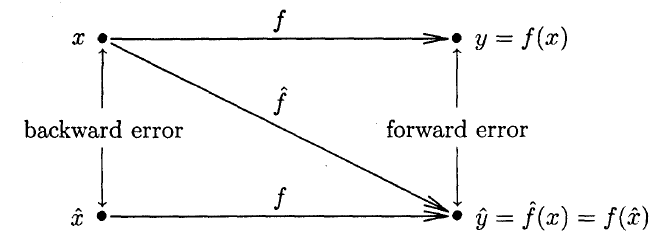
\includegraphics[width=0.5\textwidth]
	{schematic_diagram_of_forward_and_backward_error}
\end{wrapfigure}
\itmlthr{
	\item $x,f$:\@ exact input and func.\@
	\item $\hat{f}$:\@ approx.\@ func.\@
	\item $\hat{x}$:\@ exact val.\@ for $\hat{f}$ \\ \\ \\ \\ \\ \\ \\
}

\lvs
\itmltwo{
	\item $\hat{f}(x)=f(\hat{x})$ due to the choice of $\hat{x}$, which
	defines $\hat{x}$
	\item back.\@ err.\@ anly is easier, used to measure algo.\@ stability
	\item comp.\@ err.\@ $ \left\langle
		\begin{array}{lcl}
			\text{trunc.\@ err.\@} & : & \text{due to trunc.\@ of inf.\@
			series, finite diff., \ldots} \\
			\text{round.\@ err.\@} & : & \text{due to finite-precs.,
			rounding arith., \ldots}
		\end{array}
	\right.$
	\item $\tbf{total err.\@} = \hat{f}(\hat{x})-f(x) =
	\underbrace{\fbt{\hat{f}(\hat{x})-f(\hat{x})}}_{\text{comp.\@ err.\@}} +
	\underbrace{\big(f(\hat{x})-f(x)\big)}_{\text{data err.\@}}$
}

\tbl{Cond.\@ Num.\@}
\mvs{1em}
\[
	\textrm{cond} \;\frdbs{\triangleq}\; \dfrac{\fvt{\text{rel.\@ change in
	sol.\@}}}{\fvt{\text{rel.\@ change in input}}} =
	\dfrac{\big(f(\hat{x})-f(x)\big)/f(x)}{\fbt{\hat{x}-x}/x} =
	\dfrac{\fvt{\Delta y/y}}{\fvt{\Delta x/x}}
\]
\tvs
\begin{wrapfigure}{r}{0.4\textwidth}
	\centering
	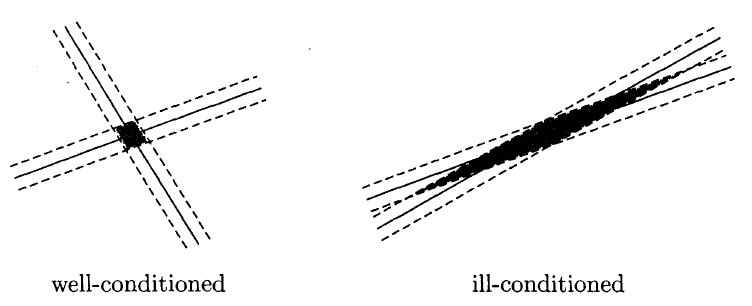
\includegraphics[width=0.4\textwidth]
	{well_conditioned_and_ill_conditioned_linear_system}
\end{wrapfigure}
\itmltwo{
	\item $\textrm{cond} \geq 1\;(>10)$: sensi./ill-cond.\@ prob.\@
	\item $\fvt{\text{rel.\@ fore.\@ err.\@}} \lessapprox \textrm{cond}
	\cdot \fvt{\text{rel.\@ back.\@ err.\@}}$
	\itmind{\item[$\circ$] $\textrm{cond}$ $\Llr$ amplification factor}
	\itmind{\item[$\circ$] $\lessapprox$:\@ \trdbf{upper bound} for the
	max.\@ cond.\@}
	\item $\textrm{cond} \approx \fvt{\dfrac{xf'(x)}{f(x)}} \;
	[\ref{eq:func_cond}]$
}

\pagebreak

\tbl{Stability}
$
	\left\{
	\begin{array}{ll}
		\underset{\text{(well-posed)}}{\text{math prob.\@}} &
		\left\langle
		\begin{array}{l}
			\text{sol.\@ exists, unique, depends continuously} \\
			\text{small input change } \slashed{\leadsto} \text{ abrupt
			change in sol.\@} \\
			\text{well-posed} \neq \text{sol.\@ is insensi.\@ to pertb.\@}
		\end{array}
		\right. \\
		\underset{\text{(stable)}}{\text{algo.\@ desp.\@}} &
		\left\langle
		\begin{array}{l}
			\text{rst.\@ rel.\@ insensi.\@ to pertb.\@ due to approx.\@} \\
			\text{rst.\@ is the exact sol.\@ to a \trdbf{nearby} prob.\@} \\
			\text{weaker:\@ \uwave{nearly} correct rst.\@ for \uwave{nearly}
			the correct prob.\@} \\
		\end{array}
		\right.
	\end{array}
	\right.
$

\tbl{Accuracy}
$
	\left\{
	\begin{array}{l}
		\text{closeness of comp.\@ sol.\@ to true sol.\@} \\
		\text{depends on algo.\@ cond.\@ and stability} \\
		\text{stability} \;\frdbs{\neq}\; \text{accuracy} \\
	\end{array}
	\right.
$
\begin{tabular}{c|c|c}
	~ & alog.\@ & prob.\@ \\
	\hline
	\multirow{2}{*}{inaccuracy} & stable & ill-cond.\@ \\
	& unstable & well-cond.\@ \\
	\hline
	accuracy & stable & well-cond.\@ \\
\end{tabular}

\tbl{Mach.\@ Precs.\@}
$
	\left\{
	\begin{array}{l}
		\vep_m = \arg\min_\vep \textrm{fl}(1+\vep)>1 \\
		\fvt{\dfrac{\textrm{fl}(x)-x}{x}} \leq \vep_m \\
	\end{array}
	\right.
$
\itmltwo{
	\item $\textrm{fl}(x)$:\@ round to nearest, $\textrm{fl}(x \oplus y)=(x
	\oplus y)(1+\delta) \esp \fvt{\delta} \leq \vep_m$
	\item $\vep_m$ determines the \uwave{max.\@ rel.\@ err.\@} in
	representing a real num.\@ $x$
}

\tbl{Err.\@ Anly.\@ Sum.\@}
\tvs
\begin{center}
\begin{tabular}{|c|c|c|c|}
	\cline{1-4}
	\multirow{3}{*}{~} & \multicolumn{3}{c|}{\trdbf{Total Err.}\@} \\
	\cline{2-4}
	~ & \multicolumn{2}{c|}{comp.\@ err.\@} & \multirow{2}{*}{data err.\@}
	\\ \cline{2-3}
	~ & trunc.\@ err.\@ & round.\@ err.\@ & ~ \\ \cline{1-4}
	\multirow{2}{*}{howto est.\@} & \multirow{2}{*}{theoretical anly.\@} &
	back.\@ err.\@ anly.\@ & \multirow{2}{*}{cond.ing,\@
	\uwave{$\textrm{cond}$}} \\
	~ & ~ & hard to quantify & ~ \\ \cline{1-4}
	\multirow{2}{*}{howto rdc.\@} & \multirow{2}{*}{aglo.\@ selction} &
	\trdbf{stable} algo.\@ & change prob.\@ form.\@ \\
	~ & ~ & tips{$^\dagger$}, dbl-precs.\@ & improve cond.ing \\ \cline{1-4}

\end{tabular}
\end{center}
\itmltwo{
	\item avoid \uwave{subtractive cancellation} in nums.\@ of nearly equal
	mag.\@
	\item avoid adding \uwave{large and small} nums.\@
	\item adjust the \uwave{order} of additions
}

\tbl{Mat.\@ Cond.\@}
\mvs{1em}
\[
	\kappa(\fbs{A}) \triangleq \fVt{\fbs{A}} \cdot \fnVt{\fbs{A}^{-1}}
\]
\tvs
\itmltwo{
	\item $\kappa$ is def.\@ for \uwave{sqr.\@ non-singlr.\@ mat.},
	$\kappa(\fbs{A})=\infty$ if $\fbs{A}$ singlr.\@
	\item $\kappa(\fbs{A}) \geq 1$, $\kappa(\fbs{I})=1$,
	$\kappa(\gamma\fbs{A})=\kappa(\fbs{A})$,
	$\kappa(\fbs{D})=\fbt{\max\fvt{d_i}}\big/\fbt{\min\fvt{d_i}},\fbs{D} =
	\textrm{diag}(d_i)$
}

\tbl{Err.\@ Bounds}
\mvs{1em}
\[
	\dfrac{\fVt{\Delta\fbs{x}}}{\fVt{\fbs{x}}} \lessapprox \kappa_1(\fbs{A})
	\dfrac{\fVt{\Delta\fbs{b}}}{\fVt{\fbs{b}}} \;[\ref{eq:b_perb_cond}] \qsp
	\dfrac{\fVt{\Delta\fbs{x}}}{\fVt{\hat{\fbs{x}}}} \lessapprox
	\kappa_2(\fbs{A}) \dfrac{\fVt{\fbs{E}}}{\fVt{\fbs{A}}}
	\;[\ref{eq:A_perb_cond}] \qsp
	\dfrac{\fVt{\Delta\fbs{x}}}{\fVt{\fbs{x}}} \lessapprox \kappa_3(\fbs{A})
	\fbt{\dfrac{\fVt{\Delta\fbs{b}}}{\fVt{\fbs{b}}} +
	\dfrac{\fVt{\fbs{E}}}{\fVt{\fbs{A}}}} \;[\ref{eq:Ab_perb_cond}]
\]
\tvs
\itmltwo{
	\item $\frdbs{\lessapprox}$:\@ approx.\@ bounded by
	\item $\kappa$ provides a quantitative bound for the err.\@ in comp.\@
	sol.\@
	\item $\kappa_1$ bounds the \uwave{max.\@ rel.\@ change in sol.}\@ due
	to a given rel.\@ change \uwave{in vec.\@ $\fbs{b}$}
	\item similar rst.\@ $\kappa_2$ holds for rel.\@ change \uwave{in mat.\@
	$\fbs{A}$}
	\item mat.\@ scaling affects $\kappa$ rather than the singlr.\@
	\item $\dfrac{\fVt{\hat{\fbs{x}}-\fbs{x}}}{\fVt{\fbs{x}}} \lessapprox
	\kappa(\fbs{A})\vep_m$ if input data accurate to mach.\@ precs.\@
}

\tbl{Residual}
$
	\left\{
	\begin{array}{l}
		\fbs{r} = \fbs{b} - \fbs{A}\hat{\fbs{x}} \text{ where }
		\hat{\fbs{x}} \text{ is approx.\@ sol.\@} \\
		\text{rel.\@ res.\@} \;\frdbs{\triangleq}\;
		\dfrac{\fVt{\fbs{r}}}{\fVt{\fbs{A}} \cdot \fVt{\hat{\fbs{x}}}}
	\end{array}
	\right.
$
\[
	\dfrac{\fVt{\Delta\fbs{x}}}{\fVt{\hat{\fbs{x}}}} \leq \kappa(\fbs{A})
	\dfrac{\fVt{\fbs{r}}}{\fVt{\fbs{A}} \cdot \fVt{\hat{\fbs{x}}}}
	\;[\ref{eq:rel_res_cond}]
\]
\tvs
\itmltwo{
	\item \uwave{size of res.\@} is considered rel.\@ to the size of prob.\@
	and sol.\@
	\item small rel.\@ res.\@ $\leadsto$ small rel.\@ err.\@ \ifof $\fbs{A}$
	is well-cond.\@
	\item large rel.\@ res.\@ $\leadsto$ large back.\@ err.\@ in mat.\@
	$\leadsto$ unstable algo.\@ $[\ref{eq:A_perb_rel_res}]$
	\item stable algo.\@ $\Llr$ small rel.\@ res.\@ (irresp.\@ to cond.ing)
}

\tbl{Tri.\@ Lin.\@ Sys.\@}
\itmlone{
	\item \tbf{lower} tri.\@ sys.\@ $ \left\langle\;
		\begin{aligned}
			& \fbs{Ly}=\fbs{b} \\
			& y_1 = b_1\big/l_{11} \qsp
			y_i=\fbt{b_i-\sum_{j=1}^{i-1}l_{ij}y_j}\Big/l_{ii} \esp
			i=2,\cdots,n \\
		\end{aligned}
	\right.$
}
\tvs
\begin{algo}[!h]{-5em}
	\caption{Fore.\@ Subs.\@ for Unit Lower Tri.\@ Mat.\@}
	$y_1 \gets b_1$\;
	\For{$i \gets 2$ \KwTo $n$}{
		$s \gets b_i$\;
		\For{$j \gets 1$ \KwTo $i-1$}{
			$s \gets s-l_{ij} \cdot y_j$\;
		}
		$y_i \gets s$
	}
\end{algo}
\mvs{1em}
\itmlone{
	\item \tbf{upper} tri.\@ sys.\@ $ \left\langle\;
		\begin{aligned}
			& \fbs{Ux}=\fbs{y} \\
			& x_n = y_n\big/u_{nn} \qsp
			x_i=\fbt{y_i-\sum_{j=i+1}^{n}u_{ij}x_j}\Big/u_{ii} \esp
			i=n-1,\cdots,1
		\end{aligned}
	\right.$
}
\tvs
\begin{algo}[!h]{-5em}
	\caption{Back.\@ Subs.\@ for Upper Tri.\@ Mat.\@}
	$x_n \gets y_n/u_{nn}$\;
	\For{$i \gets n-1$ \KwTo $1$}{
		$s \gets y_i$\;
		\For{$j \gets i+1$ \KwTo $n$}{
			$s \gets s-u_{ij} \cdot x_j$\;
		}
		$x_i \gets s/u_{ii}$
	}
\end{algo}

\mvs{3em}
\tbl{Perm.\@ Mat.\@}
\mvs{1em}
\[
	\uwave{\fbs{P}^{-1}=\fbs{P}^T} \qsp \fVt{\fbs{P}}=1 \qsp
	\kappa(\fbs{P})=1 \qsp \kappa(\fbs{PA})=\kappa(\fbs{A})
\]
\mvs{-1em}
\itmltwo{
	\item $\fbs{P}$ is sqr.\@ mat.\@ with only one $1$ in each row/col.\@
	and is always non-singlr.\@
	\item $\fbs{P}$ is orthogonal mat., prod.\@ of $\fbs{P}$ is also perm.\@
	mat.\@
	\item $\fbs{PA}$ reorders rows, $\fbs{AP}$ reorders cols.\@
}

\tbl{Elem.\@ Elim.\@ Mat.\@}
\mvs{1em}
\[
	\fbs{M}_k\fbs{a} =
	\begin{pmatrix}
		1 & \cdots & 0 & 0 & \cdots & 0 \\
		\vdots & \ddots & \vdots & \vdots & \ddots & \vdots \\
		0 & \cdots & 1 & 0 & \cdots & 0 \\
		0 & \cdots & -m_{k+1} & 1 & \cdots & 0 \\
		\vdots & \ddots & \vdots & \vdots & \ddots & \vdots \\
		0 & \cdots & -m_n & 0 & \cdots & 1 \\
	\end{pmatrix}
	\begin{pmatrix}
		a_1 \\ \vdots \\ a_k \\ a_{k+1} \\ \vdots \\ a_n
	\end{pmatrix} =
	\begin{pmatrix}
		a_1 \\ \vdots \\ a_k \\ 0 \\ \vdots \\ 0
	\end{pmatrix} \esp
	\begin{aligned}
		& m_i=a_i/a_k \\
		& i=k+1,\cdots,n \\
	\end{aligned}
\]
\itmltwo{
	\item $\fbs{M}_k$ is \uwave{unit lower tri.}, non-singlr., annihilates
	all entries below \trdbf{pivot} $a_k \neq 0$
	\item $\left.
		\begin{aligned}
			& \fbs{M}_k=\fbs{I}-\fbs{me}_k^T \\
			& \fbs{M}^{-1}_k=\fbs{I}+\fbs{me}^T_k \;\frdbs{\triangleq}\;
			\fbs{L}_k \\
		\end{aligned}
		\;\right\rangle\;
		\underset{\fbs{m}=\fbt{0,\cdots,0,m_{k+1},\cdots,m_n}^T}{\text{rever
		sed signs of multipliers}}$
	\item $\fbs{M}_k\fbs{M}_j\;(j>k)$ is their "union", and similar rst.\@
	holds for $\fbs{L}_k\fbs{L}_j\;[\ref{eq:lu_mkmj_lklj}]$
}

\tbl{$\fbs{LU}$ Fact.\@ by Gauss.\@ Elim.\@}
\mvs{1em}
\[
	\underbrace{\fbs{M}_{n-1} \cdots \fbs{M}_1}_{\text{lower tri.\@
	mat.\@}\fbs{M}}\fbs{Ax} =
	\overbrace{\underbrace{\fbs{MA}}_{\fbs{U}}\fbs{x} =
	\underbrace{\fbs{Mb}}_{\fbs{y}}}^{\text{upper tri.\@ sys.\@}} \qsp
	\fbs{LUx}=\fbs{b} \;
	\left\langle
		\begin{array}{lcl}
			\fbs{Ly}=\fbs{b} & : & \text{fore.\@ subs.\@} \\
			\fbs{Ux}=\fbs{y} & : & \text{back.\@ subs.\@} \\
		\end{array}
	\right. \;[\ref{eq:lu_l1ln1}]
\]
\itmltwo{
	\item $\fbs{LU}$ Fact.\@ is unique \;$\frdbs{\Llr}$\; $
		\left\langle
		\begin{array}{l}
			\fbs{L} \text{ is unit lower tri., } \fbs{U} \text{ is upper
			tri.\@} \\
			\text{all \uwave{leading principle submats.\@} are
			non-singlr.\@}
		\end{array}
		\right.
	$
	\item Gauss.\@ Elim.\@ and $\fbs{LU}$ Fact.\@ are two ways of expressing
	same process
	\item zero pivot causes breakdown $\leadsto$ chooes entry with large
	mag.\@
}

\tbl{Pivoting}
\mvs{1em}
\itmlone{
	\item \tbf{partial} pvt.\@
}
\itmltwo{
	\item $\fbs{M}^{-1}$ is \uwave{not necessarily} lower tri.\@ due to
	perm.\@
	\item $\fbs{PA}=\fbs{LU}$ where $\fbs{P}=\fbs{P}_{n-1} \cdots
	\fbs{P}_1$, but can't be determined in advance
	\item universally used since \tbf{N.S.}\@ is more than adaquate
}
\itmlone{
	\item \tbf{complete} pvt.\@
}
\tvs
\itmltwo{
	\item entire remaining unreduced submats.\@ is searched for the max.\@
	mag.\@
	\item $\fbs{PAQ}=\fbs{LU}$, theoretically superior, but much expensive
}

\pagebreak

\tbl{$\fbs{LU}$ Fact.\@ Stability}
\mvs{1em}
\[
	\dfrac{\fVt{\fbs{r}}}{\fVt{\fbs{A}} \cdot \fVt{\hat{\fbs{x}}}} \leq
	\dfrac{\fVt{\fbs{E}}}{\fVt{\fbs{A}}} \leq \rho\,n\,\vep_m \quad
	[\ref{eq:A_perb_rel_res}],\cite{Wilkinson:1961:EAD:321075.321076}\;
\]
\tvs
\itmltwo{
	\item $\fbs{E}$:\@ back.\@ err.\@ of mat.\@ $\fbs{A}$
	\item growth fac.\@ $\rho \;\frdbs{\triangleq}\; \dfrac{\text{max.\@
	ele.\@ of }\fbs{U}}{\text{max.\@ ele.\@ of }\fbs{A}} \;\left\langle
		\begin{array}{lcl}
			\text{without pvt.\@} & : & \text{arbitrarily large} \leadsto
			\text{unstable} \\
			\text{partial pvt.\@} & : & \rho\leq2^{n-1}\;(<10)\leadsto
			\text{stable} \\
			\text{complete pvt.\@} & : & \rho \text{ much smaller but not
			worth}
		\end{array}
	\right.$
	\item $\dfrac{\fVt{\fbs{E}}}{\fVt{\fbs{A}}} \lessapprox n\,\vep_m$ in
	practice $\overset{\text{always}}{\leadsto}$ small res.\@ regardless of
	cond.ing
	\item small res.\@ $\slashed{\Llr}$ accurate sol.\@ unless $\fbs{A}$ is
	well-cond.\@
}

\tbl{$\fbs{LU}$ Fact.\@ Algo.\@}
\begin{algo}[!h]{-5em}
	\caption{$\fbs{LU}$ Fact.\@ with Partial PVT.\@}
	\label{algo:lu_ppvt}
	$\fbs{p} \gets [1:n]$ \tcp*{aux.\@ vec.\@}
	\For{$i \gets 1$ \KwTo $n-1$}{
		$a_{ki} \gets \max_{i \leq j \leq n}\fvt{a_{ji}}$ \tcp*{find pvt.\@}
		\If{$k \neq i$}{
			\For{$j \gets 1$ \KwTo $n$}{
				$t \gets a_{ij},\; a_{ij} \gets a_{kj},\; a_{kj} \gets t$
				\tcp*{row $i$ $\rightleftharpoons$ row $k$}
			}
			$\fbs{p}(k) \gets i,\; \fbs{p}(i) \gets k$ \tcp*{upd.\@
			$\fbs{p}$}
		}
		\For{$j \gets i+1$ \KwTo $n$}{
			$a_{ji} \gets a_{ji}/a_{ii}$ \tcp*{calc.\@ col.\@ $i$}
		}
		\For{$j \gets i+1$ \KwTo $n$}{
			\For{$k \gets i+1$ \KwTo $n$}{
				$a_{jk} \gets a_{jk}-a_{ji} a_{ik}$ \tcp*{upd.\@
				$\fbs{A}[i+1:n,i+1:n]$}
			}
		}
	}
\end{algo}
\tvs
\itmltwo{
	\item fact.\@ effectively \uwave{in-place}
	\item trans.\@ of $\fbs{b}$ can be included or as a sep.\@ step
}
\itmlone{
	\item storage anly.\@ $ \left\{\begin{array}{l}
		\fbs{L},\fbs{U} \text{ overwrite init.\@ mat.\@ } \fbs{A}
		\;\left\langle\; \begin{aligned}
			\fbs{U} & \text{ on upper tri.\@} \\
			\fbs{L} & \text{ on \uwave{strict} lower tri.\@} \\
		\end{aligned} \right. \\
		\text{aux.\@ vec.\@ } \fbs{p} \text{ keeps track of new row order}
		\\
	\end{array}\right.$
	\item complexity anly.:\@
	$\dfrac{2}{3}n^3+\fsp{O}(n^2)\;[\ref{eq:lu_ppvt_comp}]$
}

\tbl{Special Lin.\@ Sys.\@}
$
	\left\{
	\begin{array}{lcl}
		\text{symm./herm.\@} & : & \fbs{A}=\fbs{A}^T,\; \fbs{A}=\fbs{A}^H \\
		\text{pos.\@ def.\@} & : & \forall\fbs{x} \neq 0 \;\;
		\fbs{x}^T\fbs{Ax}>0,\; \fbs{x}^H\fbs{Ax}>0 \\
		\text{banded} & : & \forall\fvt{i-j}>\beta \;\; a_{ij}=0, \text{
		where } \beta \triangleq \text{bandwidth} \\
		\text{sparse} & : & \text{most are zeros} \\
	\end{array}
	\right.
$

\tbl{Symm.\@ Pos.\@ Def.\@ Sys.\@}
$
	\left\{
	\begin{array}{l}
		\text{all eigvals.\@ are pos.\@} \\
		\text{all leading principle mats.\@ are \tbf{SPD}} \\
		\text{all elems.\@ on diag.\@ are pos.\@, and } \dsp
		\uwave{\max_i\{a_{ii}\} > \max_{i \neq j}\{\fvt{a_{ij}}\}} \\
		\trdbf{Cholesky Fact.:\@ } \fbs{A}=\fbs{LL}^T \\
	\end{array}
	\right.
$

\tbl{Cholesky Fact.\@}
\itmlone{
	\item $\fbs{A}=\fbs{LL}^T$
}
\evs
\[
	\begin{pmatrix}
		a_{11} & a_{12} & \cdots & a_{1n} \\
		a_{21} & a_{22} & \cdots & a_{2n} \\
		\vdots & \vdots & \ddots & \vdots \\
		a_{n1} & a_{n2} & \cdots & a_{nn} \\
	\end{pmatrix} =
	\begin{pmatrix}
		l_{11} & ~ & ~ & ~ \\
		l_{21} & l_{22} & ~ & ~ \\
		\vdots & \vdots & \ddots & ~ \\
		l_{n1} & l_{n2} & \cdots & l_{nn} \\
	\end{pmatrix}
	\begin{pmatrix}
		l_{11} & l_{21} & \cdots & l_{n1} \\
		~ & l_{22} & \cdots & l_{n2} \\
		~ & ~ & \ddots & \vdots \\
		~ & ~ & ~ & l_{nn} \\
	\end{pmatrix}
\]
\[
	a_{ij} = \sum_{k=1}^n l_{ik} l_{jk} = l_{jj} l_{ij} + \sum_{k=1}^{j-1}
	l_{ik} l_{jk} \esp i,j=1,2,\cdots,n
\]
\tvs
\begin{algo}[!h]{-5em}
	\caption{Cholesky $\fbs{LL}^T$ Fact.\@}
	\label{algo:chol_ll_fact}
	\For{$j \gets 1$ \KwTo n}{
		$a_{jj} \gets \fbt{a_{jj}-\sum_{k=1}^{j-1} a_{jk}^2}^{1/2}$
		\tcp*{diag.\@ elem.\@}
		\For{$i \gets j+1$ \KwTo $n$}{
			$a_{ij} \gets \fbt{a_{ij}-\sum_{k=1}^{j-1}a_{ik}a_{jk}}/a_{jj}$
			\tcp*{elems.\@ below diag.\@ elem.\@}
		}
	}
\end{algo}
\tvs
\itmltwo{
	\item $\fbs{A}=\fbs{LL}^T$ is unique when diag.\@ ele.\@ are required to
	be pos.\@
	\item sqr.\@ roots are all of pos.\@ $\leadsto$ algo is well-def.\@
	$\leadsto$ \uwave{no pvt.}\@ for \tbf{N.S.}:\@ $\rho \leq 1 \;
	[\ref{eq:chol_fact_growth_factor}]$
	\item only access, store, \uwave{overwrite lower} tri.\@ mat.\@ of
	$\fbs{A}$
	\item $\dfrac{1}{3}n^3+\fsp{O}(n^2) \; [\ref{eq:chol_fact_complexity}]$
	(half of $\fbs{LU}$ fact.\@); \fbox{mcmd.:\@ \tbf{chol}($\fbs{A}$)}
}
\itmlone{
	\item $\fbs{A}=\fbs{LDL}^T$
}
\evs
\[
	\begin{pmatrix}
		a_{11} & a_{12} & \cdots & a_{1n} \\
		a_{21} & a_{22} & \cdots & a_{2n} \\
		\vdots & \vdots & \ddots & \vdots \\
		a_{n1} & a_{n2} & \cdots & a_{nn} \\
	\end{pmatrix} =
	\begin{pmatrix}
		1 & ~ & ~ & ~ \\
		l_{21} & 1 & ~ & ~ \\
		\vdots & \ddots & \ddots & ~ \\
		l_{n1} & \cdots & l_{n,n-1} & 1 \\
	\end{pmatrix}
	\begin{pmatrix}
		d_1 & & & \\
		& d_2 & & \\
		& & \ddots & \\
		& & & d_n \\
	\end{pmatrix}
	\begin{pmatrix}
		1 & l_{21} & \cdots & l_{n1} \\
		~ & 1 & \cdots & l_{n2} \\
		~ & ~ & \ddots & \vdots \\
		~ & ~ & ~ & 1 \\
	\end{pmatrix}
\]
\[
	a_{ij} = \sum_{k=1}^n l_{ik} d_{k} l_{jk} =
	d_j l_{ij} + \sum_{k=1}^{j-1} l_{ik} d_{k} l_{jk} \esp
	i,j=1,2,\cdots,n
\]
\tvs
\begin{algo}[!h]{-5em}
	\caption{Cholesky $\fbs{LDL}^T$ Fact.\@}
	\label{algo:chol_ldl_fact}
	\For{$j \gets 1$ \KwTo n}{
		$a_{jj} \gets a_{jj}-\sum_{k=1}^{j-1} a_{jk}^2 a_{kk}$
		\tcp*{diag.\@ elem.\@}
		\For{$i \gets j+1$ \KwTo $n$}{
			$a_{ij} \gets
			\fbt{a_{ij}-\sum_{k=1}^{j-1}a_{ik}a_{kk}a_{jk}}/a_{jj}$
			\tcp*{elems.\@ below diag.\@ elem.\@}
		}
	}
\end{algo}
\tvs
\itmltwo{
	\item advantage of not requiring any sqr.\@ roots.
	\item $d_i$ in $\fbs{LDL}^T$ is the sqr.\@ of $l_{ii}$ in $\fbs{LL}^T$
}

\tbl{Symm.\@ inDef.\@ Lin.\@ Sys.\@}
\itmltwo{
	\item $\rho_{chol} \gg 1$ $\leadsto$ breakdown using Cholesky fact.\@
	$\leadsto$ unstable algo.\@
	\item pvt.\@ $\leadsto$ asymm.\@ $\overset{\text{exchange
	both}}{\underset{\text{rows \& cols.\@}}{\frdbs{\leadsto}}}$ symm.:\@
	$\fbs{PAP}^T=\fbs{LDL}^T$
	\item stable $\left\langle \begin{array}{lcl}
	\fbs{PAP}^T=\fbs{L}\underset{\frdbs{\cdots}}{\fbs{T}}\fbs{L}^T & , &
	\fbs{T} \text{ is symm.\@ tri.\@ mat.\@} $\;\cite{aasen1971reduction}$
	\\
	\fbs{PAP}^T=\fbs{L}\underset{\frdbs{\cdots}}{\tilde{\fbs{D}}}\fbs{L}^T &
	, & \tilde{\fbs{D}} \text{ is block tridiag.\@ mat.\@} \left\langle
	\begin{array}{l} \fts{1}{1} \\ \fts{2}{2} \end{array}\right.
	\;\cite{bunch1977some}\; \end{array}\right.$
}

\pagebreak

\tbl{Tridiag.\@ Lin.\@ Sys.\@}
\mvs{1em}
\[
	\fbs{A} =
	\begin{pmatrix}
		d_1 & u_1 & ~ & ~ \\
		l_2 & \ddots & \ddots & ~ \\
		~ & \ddots & \ddots & u_{n-1} \\
		~ & ~ & l_n & d_n \\
	\end{pmatrix} \qsp
	\begin{aligned}
		&\fvt{d_1} > \fvt{u_1} > 0 \\
		&\fvt{d_n} > \fvt{l_n} > 0 \\
		&\fvt{d_i} \;\frdbs{\geq}\; \fvt{l_i}+\fvt{u_i} > 0 \\
	\end{aligned} \qquad
	\begin{array}{ll}
		\ddagger \; \frdbs{>} \;: & \text{\uwave{irr.\@ strict} diag.\@
		dom.\@ mat.\@} \\
		\ddagger \; \frdbs{\geq} \;: & \text{\uwave{irr.\@ weak} diag.\@
		dom.\@ mat.\@} \\
	\end{array}
\]
\[
	\fbs{A} =
	\begin{pmatrix}
		d_1 & u_1 & ~ & ~ \\
		l_2 & \ddots & \ddots & ~ \\
		~ & \ddots & \ddots & u_{n-1} \\
		~ & ~ & l_n & d_n \\
	\end{pmatrix} =
	\begin{pmatrix}
		\alpha_1 & & & \\
		l_2 & \alpha_2 & & \\
		& \ddots & \ddots & \\
		& & l_n & \alpha_n \\
	\end{pmatrix}
	\begin{pmatrix}
		1 & \beta_1 & & \\
		& 1 & \ddots & \\
		& & \ddots & \beta_{n-1} \\
		& & & 1 \\
	\end{pmatrix} \;\frdbs{\triangleq}\; \fbs{LU} \esp
	\begin{aligned}
		\alpha_i &= d_i - l_i\beta_{i-1} \\
		\beta_i &= u_i / \alpha_i \;(\;\uwave{\beta_0 = 0}\;)\; \\
		i &= 1,\cdots,n
	\end{aligned}
\]
\mvs{.5em}
\[
	\fbs{Ax}=\fbs{b} \Rightarrow \fbs{LUx}=\fbs{b}
	\;\left\langle
		\begin{array}{lclcl}
			\fbs{Ly}=\fbs{b} & \Rightarrow &
			y_i=\fbt{b_i-l_iy_{i-1}}/\alpha_i & , & i=1,\cdots,n \esp
			\uwave{y_0=0} \\
			\fbs{Ux}=\fbs{y} & \Rightarrow & x_i= \fbt{y_i-\beta_ix_{i+1}} &
			, & i=n,\cdots,1 \esp \uwave{x_{n+1}=0}\\
		\end{array}
	\right.
\]
\tvs
\begin{algo}[!h]{-5em}
	\caption{Thomas Algo.\@ for Tridiag.\@ Lin.\@ Sys.\@}
	\label{algo:thomos_tridiag_lin_sys}
	$\beta_0=0,\; y_0=0,\; x_{n+1}=0$
	\tcp*{init.\@ val.\@}
	\For{$i \gets 1$ \KwTo $n$}{
		$\alpha_i \gets d_i - l_i\beta_{i-1}$
		\tcp*{calc.\@ $\alpha_i$}
		$\beta_i \gets u_i/\alpha_i$
		\tcp*{calc.\@ $\beta_i$}
		$y_i \gets \fbt{b_i-l_iy_{i-1}}/\alpha_i$
		\tcp*{calc.\@ $y_i$}
	}
	\For{$i \gets n$ \KwTo $1$}{
		$x_i \gets (y_i-\beta_ix_{i+1})$
		\tcp*{calc.\@ $x_i$}
	}
\end{algo}
\tvs
\itmltwo{
	\item $0 < \fvt{\beta_i} < 1$ $\frdbs{\leadsto}$ err.\@ in back.\@
	subs.\@ is under control
	\item $0 < \fvt{d_i}-\fvt{l_i} < \fvt{\alpha_i} < \fvt{d_i}+\fvt{l_i}
	\esp i=2,3,\cdots,n$ $\frdbs{\leadsto}$ $\alpha_i\neq0$
	\item solve $\fbs{Ly}=\fbs{b}$ and $\fbs{LU}$ fact.\@ simultaneously
	$\leadsto$ no need to store $\alpha_i$ but $\beta_i$
	\item complexity:\@ $8n \;[\ref{eq:thomas_tridiag_complexity}]$
}

\tbl{Banded Tri.\@ Lin.\@ Sys.\@}
\mvs{1em}
\[
	a_{ij} = 0 \quad \text{for}
	\; \left\{ \;
		\begin{aligned}
			i & > j + b_{L} \\
			i & < j - b_{U} \\
		\end{aligned}
	\right.
\]
\begin{figure}[h]
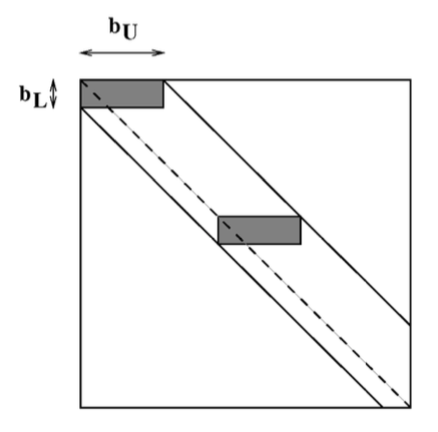
\includegraphics[width=0.25\linewidth]{banded_matrix}
\centering
\end{figure}
\itmlone{
	\item $\underset{(\fbs{A}=\fbs{LU})}{\text{no pvt.\@}} \; \left\langle
	\begin{array}{lcl} \fbs{L} & : & \text{lower band}=b_{L} \\ \fbs{U} & :
		& \text{upper band}=b_{U} \end{array}\right.$
	\item $\underset{(\fbs{PA}=\fbs{LU})}{\text{partial pvt.\@}} \;
	\left\langle \begin{array}{lcl} \fbs{L} & : & \text{lower band}=b_{L}
	\text{ with at most $b_{L}+1$ nz.\@ in each col.\@}\\ \fbs{U} & : &
	\text{upper band} \leq b_{L}+b_{U} \end{array}\right.$
}
\itmltwo{
	\item complexity:\@ $2nb_Lb_U+2n(b_L+b_U)$
}

\pagebreak

\tbl{Pertb.\@ Anly.\@}
\mvs{1em}
\[
	\left. \begin{aligned}
		\fbs{Ax} &= \fbs{b} \\
		(\fbs{A}+\fbs{\delta A})\fbs{x}^\ast &= \fbs{b} + \fbs{\delta b} \\
		\fbs{r} &= \fbs{b}-\fbs{Ax}^\ast \\
	\end{aligned} \; \right\}
	\; \underset{\text{back.\@ anly.\@}}{\frdbs{\Longrightarrow}} \;
	\begin{aligned}
		\fbs{\delta x} &= \fbs{x}^\ast - \fbs{x} \\
		&= -\fbs{A}^{-1}\fbs{r} \;[\ref{eq:pertb_delta_res}] \\
	\end{aligned} \quad
	\left\{ \begin{array}{lcl}
		\fbs{x} & : & \text{exact sol.\@} \\
		\fbs{x}^\ast & : & \text{approx.\@ sol.} \\
		\fbs{r} & : & \text{res.} \\
	\end{array} \right.
\]
\tvs
\itmlone{
	\item $\fbs{\delta x} \;\frdbs{\leftrightsquigarrow}\; \fbs{x}^\ast$
	($\fbs{A}$ is non-singlr.\@)
}
\evs
\[
	\dfrac{\fVt{\fbs{\delta x}}}{\fVt{\fbs{x}^\ast}} \leq
	\fnVt{\fbs{A}^{-1}} \cdot \fVt{\fbs{A}} \cdot \fbt{
		\dfrac{\fVt{\fbs{\delta A}}}{\fVt{\fbs{A}}} +
		\dfrac{\fVt{\fbs{\delta b}}}{\fVt{\fbs{A}} \cdot \fVt{\fbs{x}^\ast}}
	} \;[\ref{eq:pertb_delta_approx}]
\]
\[
	\dfrac{\fVt{\fbs{\delta x}}}{\fVt{\fbs{x}^\ast}} \leq \kappa(\fbs{A})
	\cdot
	\dfrac{\fVt{\fbs{\delta A}}}{\fVt{\fbs{A}}} \text{ when }
	\fVt{\fbs{\delta b}}=0
\]
\itmlone{
	\item $\fbs{\delta x} \;\frdbs{\leftrightsquigarrow}\; \fbs{x}$
	($\fbs{A}$ is non-singlr.,\@ $\uwave{\fnVt{\fbs{A}^{-1}} \cdot
	\fVt{\delta \fbs{A}} < 1}$)
}
\evs
\[
	\dfrac{\fVt{\fbs{\delta x}}}{\fVt{\fbs{x}}} \leq
	\dfrac{\kappa(\fbs{A})}{1-\kappa(\fbs{A}) \cdot \dfrac{\fVt{\fbs{\delta
	A}}}{\fVt{\fbs{A}}}} \cdot \fbt{
		\dfrac{\fVt{\fbs{\delta A}}}{\fVt{\fbs{A}}} +
		\dfrac{\fVt{\fbs{\delta b}}}{\fVt{\fbs{b}}}
	} \;[\ref{eq:pertb_delta_exact}]
\]
\[
	\dfrac{1}{\kappa(\fbs{A})} \cdot \dfrac{\fVt{\fbs{\delta
	b}}}{\fVt{\fbs{b}}} \leq
	\dfrac{\fVt{\fbs{\delta x}}}{\fVt{\fbs{x}}} \leq
	\kappa(\fbs{A}) \cdot \dfrac{\fVt{\fbs{\delta b}}}{\fVt{\fbs{b}}}
	\text{ when } \fVt{\fbs{\delta A}}=0
\]
\itmlone{
	\item $\fbs{\delta x} \;\frdbs{\leftrightsquigarrow}\; \fbs{r}$
	($\fbs{A}$ is non-singlr.\@)
}
\evs
\[
	\fVt{\fbs{\delta x}} \leq \fnVt{\fbs{A}^{-1}} \cdot \fVt{\fbs{r}}
	\;[\ref{eq:pertb_delta_res}]
\]

\tbl{Accuracy Imprv.\@}
\itmlone{
	\item scaling
}
\tvs
\itmltwo{
	\item scale by multiplying a diag.\@ mat.\@ $\fbs{D}$:\@
	$\fbs{DADy}=\fbs{Db} \esp \fbs{x}=\fbs{Dy}$;
	\item scaling affects cond.ing; not practical but worth trying for
	ill-cond.\@ sys.\@
	\item accuracy is usually enhanced if all entries have abt.\@ same order
	of mag.\@
}
\itmlone{
	\item iter.\@ refine.\@ $ \left\{\begin{array}{l}
		\text{calc.\@ res.\@ $\fbs{r}$ for approx.\@ sol.\@ $\fbs{x}$:\@
		$\fbs{r}=\fbs{b}-\fbs{Ax}^\ast$} \\
		\text{sol.\@ } \fbs{Az}=\fbs{r} \;[\ref{eq:iter_refine_az_r}]
		\text{ with two tri.\@ lin.\@ sys.\@}
		\;[\ref{eq:iter_refine_tri_lin_sys}]: \fsp{O}(n^2)
	\end{array}\right.$
}
\tvs
\begin{algo}[!h]{-5em}
	\caption{Accuracy Enhance.\@ by Iter.\@ Refine.\@}
	let $\fbs{PA}=\fbs{LU}$, $\fbs{x}^\ast$ as approx.\@ sol.\@\;
	\Repeat{$\fbs{x}^\ast$ converges}{
		calc.\@ $\fbs{r} \gets \fbs{b}-\fbs{Ax}^\ast$\;
		sol.\@ $\fbs{Ly}=\fbs{Pr}$
		\tcp*[r]{$\fbs{y}=\fbs{L}^{-1}\fbs{Pr}$}
		sol.\@ $\fbs{Uz}=\fbs{y}$
		\tcp*[r]{$\fbs{z}=\fbs{U}^{-1}\fbs{y}$}
		$\fbs{x}^\ast \gets \fbs{x}^\ast + \fbs{z}$
		\tcp*[r]{new approx.\@ sol.\@}
    }
\end{algo}
\mvs{2em}
\itmltwo{
	\item $\fbs{x}^\ast+\fbs{z}$ is the exact sol., but $\fbs{z}^\ast$ is
	found in practice
	\item $\fVt{\fbs{r}-\fbs{Az}^\ast}$ is smaller than $\fVt{\fbs{r}}$
	$\frdbs{\leadsto}$ $\fbs{x}^\ast+\fbs{z}^\ast$ is closer to exact sol.\@
	than $\fbs{x}^\ast$
	\item $\fbs{A}$ can not be overwritten $\frdbs{\leadsto}$
	$\fbs{A},\fbs{L},\fbs{U}$ are stored
}

\pagebreak

\tbl{Lin.\@ LSQ.\@ Prob.\@}
\mvs{1em}
\[
	\fbs{Ax} \cong \fbs{b} \;\frdbs{\Leftrightarrow}\; \min_{\fbs{x} \in
	\fls{R}^n} \fVt{\fbs{b}-\fbs{Ax}}_2 = \min_{\fbs{x} \in
	\fls{R}^n} \fVt{\fbs{r}}_2 \quad
	\left\{ \begin{array}{lcl}
		m=n & : & \fbs{x}=\fbs{A}^{-1}\fbs{b} \text{ if } \fbs{A} \text{ is
		non-singlr.\@}\\
		m>n & : & \text{\trdbf{overdet.\@} (in most cases)} \\
		m<n & : & \text{underdet.\@}
	\end{array}\right.
\]
\tvs
\itmltwo{
	\item uniqueness: sol.\@ to $\fbs{Ax}\cong\fbs{b}$ is unique
	\trdbf{iff.\@} $\fbs{A}$ is \uwave{full col.\@ rank}:\@
	$\mathrm{rank}(\fbs{A})=n$
	\item existence: sol.\@ always exists but not unique if $\fbs{A}$ is
	\uwave{rank-deficient}
}

\tbl{Cond.ing of Lin.\@ LSQ.\@ Prob.\@}
\begin{wrapfigure}{r}{0.3\textwidth}
	%\centering
	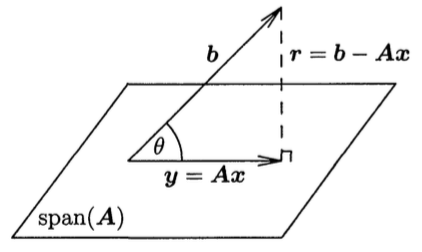
\includegraphics[width=0.2\textwidth]
	{geometric_depiction_of_linear_lsq_problem}
\end{wrapfigure}
\itmlone{
	\item \trdbf{pseudoinv.}\@ for non-singlr.\@ mat.: $
		\fbs{A}^+ \;\frdbs{\triangleq}\; (\fbs{A}^T\fbs{A})^{-1}\fbs{A}^T
	$
	\item cond.\@ num.\@ $
		\left\langle \begin{array}{lcl}
			\text{full col.\@ rank} & : & \kappa(\fbs{A})
			\;\frdbs{\triangleq}\; \fVt{\fbs{A}} \cdot \fnVt{\fbs{A}^+} \\
			\text{defective rank} & : & \kappa(A) = \infty \\
		\end{array} \right.
	$ \\ \\
}

\tbl{Sensitivity of Lin.\@ LSQ.\@ Prob.\@}
\mvs{1em}
\[
	\begin{array}{lclc}
		\underset{\fbs{b}+\Delta\fbs{b}}{\text{pertb.\@ in }\fbs{b}} & : &
		\dfrac{\fVt{\Delta\fbs{x}}}{\fVt{\fbs{x}}} \leq \kappa(\fbs{A})
		\cdot \dfrac{1}{\cos\theta} \cdot
		\dfrac{\fVt{\Delta\fbs{b}}}{\fVt{\fbs{b}}} &
		[\ref{eq:lsq_pertb_in_b}] \vspace{1em} \\
		\underset{\fbs{A}+\fbs{E}}{\text{pertb.\@ in }\fbs{A}} & : &
		\dfrac{\fVt{\Delta\fbs{x}}}{\fVt{\fbs{x}}} \lessapprox
		\fbbt{\kappa^2(\fbs{A}) \cdot \tan\theta + \kappa(\fbs{A})} \cdot
		\dfrac{\fVt{\fbs{E}}}{\fVt{\fbs{A}}} & [\ref{eq:lsq_pertb_in_a}] \\
	\end{array}
\]

\tbl{LSQ.\@ Prob.\@ Trans.\@}
\mvs{1em}
\[
	\underset{\text{overdet.\@}}{\fbs{Ax} \cong \fbs{b}}
	\;\frdbs{\leadsto}\; \text{sqr.\@ lin.\@ sys.\@}
	\;\frdbs{\leadsto}\; \text{tri.\@ lin.\@ sys.\@}
	\left\{ \begin{array}{lcl}
		\trdbf{1)\@ }\text{normal eq.\@} & : & \text{fastest} \\
		\trdbf{2)\@ }\text{QR Fact.\@} & : & \text{most important} \\
		\trdbf{3)\@ }\text{SVD Fact.\@} & : &
		\text{slowest but most reliable} \\
	\end{array} \right.
\]

\tbl{Normal Eq.\@}
\mvs{1em}
\[
	\begin{aligned}
		\fbs{A}\in\fls{R}^{\fts{m}{n}} & \;(m \geq n),\;
		\fbs{x}^\ast \in \fls{R}^n \text{ \uwave{is lsq.\@ sol.\@} }
		\trdbf{iff.\@ } \fbs{r}=\fbs{b}-\fbs{Ax}^\ast \perp
		\mathrm{Ran}(\fbs{A}) \\
		& \frdbs{\Rightarrow}\;
		\left\langle \begin{array}{lcl}
			\fbs{A}^T\fbs{Ax} = \fbs{A}^T\fbs{b} & : &
			\text{lsq.\@ prob.\@ sol.\@ $\iff$ normal eq.\@ sol.\@}\\
			\fbs{A}^T(\fbs{b}-\fbs{Ax})=0 & : &
			\text{res.\@ } \fbs{r}=\fbs{b}-\fbs{Ax}
			\text{ is \trdbf{ortho.}\@ to } \mathrm{span}(\fbs{A})
			\text{ (geo.\@ view)} \\
		\end{array}\right. \\
	\end{aligned}
\]
\tvs
\itmltwo{
	\item rect.\@ mat.\@ $\leadsto$ sqr.\@ mat.\@ $\leadsto$ tri.\@ mat.\@
	\item $
		\underset{\mathrm{rank}(\fbs{A})=n}{\fbs{A}
		\text{ is full col.\@ rank}} \Rightarrow \left\{\begin{array}{l}
			\fbs{A}^T\fbs{A} \text{ is symm.\@ pos.\@ def.\@} \\
			\text{unique lsq.\@ sol.:\@ }
			\fbs{x}=(\fbs{A}^T\fbs{A})^{-1}\fbs{A}^T\fbs{b} \\
			\text{Cholesky Fact.:\@ } \fbs{A}^T\fbs{A}=\fbs{LL}^T \Rightarrow
			\left\langle \begin{aligned}
				\fbs{Ly} &= \fbs{A}^T\fbs{b} \\
				\fbs{L}^T\fbs{x} &= \fbs{y} \\
			\end{aligned} \right.
		\end{array}\right.
	$
	\itmind{\item[$\circ$] info.\@ can be lost in forming
	$\fbs{A}^T\fbs{A}$ and $\fbs{A}^T\fbs{b}$}
	\itmind{\item[$\circ$] cond.\@ num.\@ is \tbf{sqr.}\@ of
	$\kappa(\fbs{A})$}: $\kappa(\fbs{A}^T\fbs{A})=\kappa^2(\fbs{A})$
	$\leadsto$ \trdbf{unstable algo.\@}
	\item Chol.\@ Fact.\@ complexity of $\fbs{A}^T\fbs{A}$:
	$mn^2+\dfrac{1}{3}n^3+\fsp{O}(n^2)
	\;[\ref{eq:ata_chol_fact_complexity}]$
}

\pagebreak

\tbl{$\fbs{QR}$ Fact.\@}
$
	\left\langle \begin{array}{lcl}
		\fbs{Q} & : & \text{orthornormal / unitary mat.\@} \\
		\fbs{R} & : & \text{upper tri.\@ mat} \\
	\end{array} \right. \quad \frdbs{\leadsto} \quad
	\begin{array}{c}
		\fbs{A}=\fbs{QR} \\
		(\fbs{A} \in \fls{C}^{\fts{m}{n}}, m \geq n) \\
	\end{array}
$
\itmltwo{
	\item existence:\@ $\exists\; \fbs{Q}\in\fls{C}^{\fts{m}{n}} \;
	(\fbs{Q}^\ast\fbs{Q}=\fbs{I}) \esp \fbs{R} \in \fls{C}^{\fts{n}{n}} \;
	(r_{ij}=0,i>j)$
	\item uniqueness:\@ $\fbs{QR}$ fact.\@ is unique \trdbf{iff.\@}
	$\fbs{A}$ is full col.\@ rank, and $r_{ii}>0$
	\item app:\@ $^{1)\,}$lin.\@ lsq.\@ prob.\@; $^{2)\,}$eigval.\@ prob.\@;
	$^{3)\,}$$\fbs{Ax}=\fbs{b}$ when $\fbs{A}$ is non-singlr.\@ sqr.\@ mat.\@
}

\tbl{$\fbs{QR}$ Fact.\@ $\leftrightsquigarrow$ Lin.\@ LSQ.\@ Prob.\@}
\mvs{1em}
\[
	\begin{array}{c}
		\text{derv.\@ mmz.\@ of lin.\@ lsq.\@ prob.} \\
		\text{with $\fbs{QR}$ fact.\@} \\
	\end{array} \;\leadsto\;
	\left.\begin{array}{lcl}
		^{1)\;}\text{augment } \fbs{Q} & : & [\ref{eq:mmz_derv_with_aug_q}] \\
		^{2)\;}\text{trans. } \fbs{b} & : & [\ref{eq:mmz_derv_with_trans_b}] \\
		^{3)\;}\text{normal eq.\@} & : & [\ref{eq:mmz_derv_with_normal_eq}] \\
	\end{array} \;\right\rangle \;\frdbs{\Rightarrow}\;
	\fbs{x}^\ast = \fbs{R}^{-1}\fbs{Q}^T\fbs{b}
\]

\lfm{
	\label{eq:mmz_derv_with_aug_q}
	\begin{aligned}
		\left. \begin{aligned}
			& \fbs{A}_{\fts{m}{n}} = \fbs{Q}_{\fts{m}{n}} \fbs{R}_{\fts{n}{n}} \\
			& (\fbs{Q},\hat{\fbs{Q}}) \in \fls{R}^{\fts{m}{m}} \\
		\end{aligned} \;\right\rangle &\;\Rightarrow\;
		\fbVt{\fbs{Ax}-\fbs{b}}_2^2 = \fbVt{(\fbs{Q},\hat{\fbs{Q}})^T \cdot
		(\fbs{Ax}-\fbs{b})}_2^2 = \fVt{\fpm{\fbs{Q}^T \\ \hat{\fbs{Q}}^T}
		\cdot (\fbs{QRx}-\fbs{b})}_2^2 \\
		&= \fVt{\fpm{\fbs{Rx}-\fbs{Q}^Tb \\ -\hat{\fbs{Q}}^T\fbs{b}}}^2_2
		= \fbVt{\fbs{Rx}-\fbs{Q}^T\fbs{b}}_2^2 +
		\fbVt{\hat{\fbs{Q}}^T\fbs{b}}_2^2 \;\frdbs{\geq}\;
		\fbVt{\hat{\fbs{Q}}^T\fbs{b}}_2^2 \;\frdbs{\Rightarrow}\; \fbs{x}^\ast = \fbs{R}^{-1}\fbs{Q}^T\fbs{b} \\
	\end{aligned}
}

\lfm{
	\label{eq:mmz_derv_with_trans_b}
	\begin{aligned}
		& \fbs{A}_{\fts{m}{n}} = \fbs{Q}_{\fts{m}{n}} \fbs{R}_{\fts{n}{n}} \esp
		\fbs{b} = (\fbs{QQ}^T+\fbs{I}-\fbs{QQ}^T)\fbs{b} \\
		\Rightarrow\; & \fbs{Ax}-\fbs{b} = \fbs{Ax} -
		(\fbs{QQ}^T+\fbs{I}-\fbs{QQ}^T)\fbs{b} =
		(\fbs{Ax} - \fbs{QQ}^T\fbs{b}) - (\fbs{I}-\fbs{QQ}^T)\fbs{b} \\
		^\dagger{\;\frdbs{\Rightarrow}\;} &
		\fbVt{\fbs{Ax}-\fbs{b}}_2^2 = \fVt{\fbs{Ax}-\fbs{QQ}^T\fbs{b}}_2^2 +
		\fVt{(\fbs{I}-\fbs{QQ}^T)\fbs{b}}_2^2 =
		\fVt{\fbs{Q}(\fbs{Rx}-\fbs{Q}^T\fbs{b})}_2^2 +
		\fVt{(\fbs{I}-\fbs{QQ}^T)\fbs{b}}_2^2 \\
		\frdbs{\geq}\; & \fVt{(\fbs{I}-\fbs{QQ}^T)\fbs{b}}_2^2 \;\frdbs{\Rightarrow}\; \fbs{x}^\ast = \fbs{R}^{-1}\fbs{Q}^T\fbs{b} \\
	\end{aligned}
}

\lfm{
	\label{eq:mmz_derv_with_normal_eq}
	\begin{aligned}
		\fbs{x}^\ast = (\fbs{A}^T\fbs{A})^{-1}\fbs{A}^T\fbs{b} =
		(\fbs{R}^T \underbrace{\fbs{Q}^T\fbs{Q}}_{\fbs{I_{\fts{n}{n}}}}
		\fbs{R})^{-1}\fbs{R}^T\fbs{Q}^T\fbs{b} =
		\fbs{R}^{-1}\fbs{R}^{-T}\fbs{R}^T\fbs{Q}^T\fbs{b} \;\frdbs{=}\;
		\fbs{R}^{-1}\fbs{Q}^{T}\fbs{b}
	\end{aligned}
}

\tbl{}

% Appendix
%%%%%%%%%%%%%%%%%%%%%%%%%%%%%%%%%%%%%%%%%%%%%%%%%%%%%%%%%%%%%%%%%
%
% ID: formula.tex whchen
%
%%%%%%%%%%%%%%%%%%%%%%%%%%%%%%%%%%%%%%%%%%%%%%%%%%%%%%%%%%%%%%%%%


% \begin{fleqn}[⟨margin⟩] ... \end{fleqn}
% \begin{ceqn} ... \end{ceqn}
% \eq{⟨formula⟩} = \begin{equation} ⟨formula ⟩ \end{equation}
% \eqalign{⟨formulas⟩} =
% \begin{equation} \begin{darray}{rcl} ⟨formulas⟩ \end{darray} \end{equation}

\setcounter{page}{1}

\lfm{
	\label{eq:taylor_series}
	f(x) = f(a) + f'(a)(x-a) + \dfrac{f''(a)}{2!}(x-a)^2 + \dfrac{f^{(3)}(a)}{3!}(x-a)^3 + \cdots + \dfrac{f^{(n)}(a)}{n!}(x-a)^n + \cdots
}

\lfm{
	\label{eq:func_err_est}
	f(x)-f(\tilde{x}) \approx f'(\tilde{x})(x-\tilde{x}) + \dfrac{1}{2}f'(\tilde{\xi})(x-\tilde{x})^2 \underset{\fvt{e}=\fvt{x-\tilde{x}}\leq\vep}{\frdbs{\Rightarrow}}
	\begin{aligned}
		\vep\fbt{f(x)} & \leq
		\fvt{f'(\tilde{x})}\vep(x)+\dfrac{\fvt{f''(\xi)}}{2}\vep^2(x) \\
		& \lessapprox \fvt{f'(\tilde{x})}\vep(x) \underset{f'(x) \approx f'(\tilde{x})}{\frdbs{=}} \fvt{f'(x)}\vep(x)
	\end{aligned}
}

\lfm{
	\label{eq:func_cond}
	\begin{aligned}
		\dfrac{\Delta y}{y} &= \dfrac{f(x+\Delta x)-f(x)}{f(x)} \approx \dfrac{f'(x)\Delta x}{f(x)} \;\frdbs{\Rightarrow}\; \textrm{cond} \approx \dfrac{\fvt{\Delta y/y}}{\fvt{\Delta x /x}} = \dfrac{\fvt{xf'(x)}}{\fvt{f(x)}}
	\end{aligned}
}

\lfm{
	\label{eq:b_perb_cond}
	\left.
	\begin{aligned}
		& \left.
		\begin{array}{c}
			\fbs{Ax} = \fbs{b} \\
			\fbs{A}\hat{\fbs{x}} = \fbs{b} + \Delta\fbs{b}
		\end{array}
		\right\rangle \underset{\Delta\fbs{x}=\hat{\fbs{x}}-\fbs{x}}{\;\frdbs{\Rightarrow}\;} \fbs{A}\Delta\fbs{x} = \Delta\fbs{b} \\
		& \fVt{\fbs{b}} = \fVt{\fbs{Ax}} \leq \fVt{\fbs{A}} \cdot \fVt{\fbs{x}} \\
		& \fVt{\Delta\fbs{x}} = \fnVt{\fbs{A}^{-1}\fbs{b}} \leq \fnVt{\fbs{A}^{-1}} \cdot \fVt{\Delta\fbs{b}} \\
	\end{aligned}
	\;\right\} \;\frdbs{\Rightarrow}\;
	\begin{aligned}
		\dfrac{\fVt{\Delta\fbs{x}}}{\fVt{\fbs{x}}} \leq \fnVt{\fbs{A}^{-1}} \cdot \fVt{\Delta\fbs{b}} \cdot \dfrac{\fVt{\fbs{A}}}{\fVt{\fbs{b}}} = \kappa(\fbs{A}) \dfrac{\fVt{\Delta\fbs{b}}}{\fVt{\fbs{b}}}
	\end{aligned}
}

\lfm{
	\label{eq:A_perb_cond}
	\begin{aligned}
		\left.
		\begin{array}{c}
			\fbs{Ax}=\fbs{b} \\
			(\fbs{A}+\fbs{E})\hat{\fbs{x}}=\fbs{b}
		\end{array}
		\right\rangle
		& \Rightarrow \Delta{\fbs{x}} = \hat{\fbs{x}}-\fbs{x} = \fbs{A}^{-1}(\fbs{A}\hat{\fbs{x}}-\fbs{b}) = \fbs{A}^{-1}(-\fbs{E}\hat{\fbs{x}}) = - \fbs{A}^{-1}\fbs{E}\hat{\fbs{x}} \\
		& \Rightarrow \fVt{\Delta\fbs{x}} \leq \fnVt{\fbs{A}^{-1}} \cdot \fVt{\fbs{E}} \cdot \fVt{\hat{\fbs{x}}} \;\frdbs{\Rightarrow}\;
		\dfrac{\fVt{\Delta\fbs{x}}}{\fVt{\hat{\fbs{x}}}} \leq \kappa(\fbs{A}) \dfrac{\fVt{\fbs{E}}}{\fVt{\fbs{A}}} \\
	\end{aligned}
}

\lfm{
	\label{eq:Ab_perb_cond}
	\begin{aligned}
		\left.
		\begin{array}{c}
			\fbs{Ax} = \fbs{b} \\
			(\fbs{A}+\fbs{E})\hat{\fbs{x}} = \fbs{b} + \Delta\fbs{b}
		\end{array}
		\right\rangle
		& \Rightarrow \Delta\fbs{x} = \hat{\fbs{x}} - \fbs{x} = \fbs{A}^{-1}(\fbs{A}\hat{\fbs{x}}-\fbs{b}) = \fbs{A}^{-1}(\Delta\fbs{b}-\fbs{E}\hat{\fbs{x}}) \\
		& \Rightarrow \fVt{\Delta\fbs{x}} \leq \fnVt{\fbs{A}^{-1}\Delta\fbs{b}} + \fnVt{\fbs{A}^{-1}\fbs{E}\hat{\fbs{x}}} \leq \fnVt{\fbs{A}^{-1}} \cdot \fVt{\Delta\fbs{b}} + \fnVt{\fbs{A}^{-1}} \cdot \fVt{\fbs{E}} \cdot \fVt{\fbs{x}}\\
		& \;\frdbs{\Rightarrow}\; \dfrac{\Delta{\fbs{x}}}{\fVt{\fbs{x}}} \leq \dfrac{\fVt{\fbs{A}} \cdot \fnVt{\fbs{A}^{-1}} \cdot \fVt{\Delta \fbs{b}}}{\fVt{\fbs{A}} \cdot \fVt{\fbs{x}}} + \dfrac{\fVt{\fbs{A}} \cdot \fnVt{\fbs{A}^{-1}} \cdot \fVt{\fbs{E}}}{\fVt{\fbs{A}}} = \kappa(\fbs{A}) \fbt{\dfrac{\fVt{\Delta\fbs{b}}}{\fVt{\fbs{b}}} + \dfrac{\fVt{\fbs{E}}}{\fVt{\fbs{A}}}} \\
	\end{aligned}
}

\lfm{
	\label{eq:rel_res_cond}
	\left.
	\begin{aligned}
		\fVt{\Delta\fbs{x}} &= \fVt{\hat{\fbs{x}}-\fbs{x}} = \fnVt{\fbs{A}^{-1}(\fbs{A}\hat{\fbs{x}}-\fbs{b})} \\
		& \underset{\fbs{r}=\fbs{b}-\fbs{A}\hat{\fbs{x}}}{=} \fnVt{\fbs{A}^{-1}(-\fbs{r})} \leq \fnVt{\fbs{A}^{-1}} \cdot \fVt{\fbs{r}}
	\end{aligned}
	\;\right\rangle\;\frdbs{\Rightarrow}\;
	\dfrac{\fVt{\Delta\fbs{\fbs{x}}}}{\fVt{\fbs{x}}} \leq \dfrac{\fVt{\fbs{A}} \cdot \fnVt{\fbs{A}^{-1}} \cdot \fVt{\fbs{r}}}{\fVt{\fbs{A}} \cdot \fVt{\fbs{x}}} = \kappa(\fbs{A}) \dfrac{\fVt{\fbs{r}}}{\fVt{\fbs{A}} \cdot \fVt{\fbs{x}}} \\
}

\lfm{
	\label{eq:A_perb_rel_res}
	(\fbs{A}+\fbs{E})\hat{\fbs{x}} = \fbs{b} \Rightarrow \fVt{\fbs{r}} = \fVt{\fbs{b}-\fbs{A}\hat{\fbs{x}}} = \fVt{\fbs{E}\hat{\fbs{x}}} \leq \fVt{\fbs{E}} \cdot \fVt{\hat{\fbs{x}}}
	\;\frdbs{\Rightarrow}\; \dfrac{\fVt{\fbs{r}}}{\fVt{\fbs{A}} \cdot \fVt{\hat{\fbs{x}}}} \leq \dfrac{\fVt{\fbs{E}}}{\fVt{\fbs{A}}}
}

\lfm{
	\label{eq:lu_l1ln1}
	\left.
	\begin{array}{c}
		\fbs{MA}=\fbs{U} \\
		\fbs{A}=\fbs{LU} \\
	\end{array}
	\right\rangle \Rightarrow \fbs{L}=\fbs{M}^{-1} = \fbt{\fbs{M}_{n-1} \cdots \fbs{M}_1}^{-1} = \fbs{M}_1^{-1} \cdots \fbs{M}_{n-1}^{-1} \;\frdbs{=}\; \fbs{L}_1 \cdots \fbs{L}_{n-1}
}

\lfm{
	\label{eq:lu_mkmj_lklj}
	\left.\begin{aligned}
		\fbs{M}_k\fbs{M}_j &= \fbt{\fbs{I}-\fbs{me}_k^T}\fbt{\fbs{I}-\fbs{te}_j^T} = \fbs{I} - \fbs{te}_j^T - \fbs{me}_k^T + \fbs{me}_k^T\fbs{te}_j^T \;  \\
		\fbs{L}_k\fbs{L}_j &= \fbt{\fbs{I}+\fbs{me}_k^T}\fbt{\fbs{I}+\fbs{te}_j^T} = \fbs{I} + \fbs{te}_j^T + \fbs{me}_k^T + \fbs{me}_k^T\fbs{te}_j^T \;
	\end{aligned}\right\rangle
	\overset{\fbs{e}_k^T\fbs{t}=0}{\underset{\text{if }j>k}{\frdbs{=}}}
	\left\langle\begin{aligned}
		\fbs{I} - \fbs{te}_j^T - \fbs{me}_k^T \\
		\fbs{I} + \fbs{te}_j^T + \fbs{me}_k^T \\
	\end{aligned}\right.
}

\lfm{
	\label{eq:lu_ppvt_comp}
	\begin{aligned}
		\fbs{O}_{\text{lu}} = \sum_{i=1}^{n-1}\fbt{\sum_{j=i+1}^n1+\sum_{j=i+1}^n\sum_{k=i+1}^n2} = \sum_{i=1}^{n-1}\fbt{n-i+2(n-i)^2} &= \dfrac{n(n-1)}{2} + 2\dfrac{n(n-1)(2n-1)}{6} \\
		&= \dfrac{2}{3}n^3+\fsp{O}(n^2)
	\end{aligned}
}

\pagebreak

\lfm{
	\label{eq:chol_fact_growth_factor}
	\fbs{A} = \fbs{L}_0 \underbrace{\fbs{D}\fbs{L}_0^T}_{\fbs{U}} \Rightarrow \fbs{U}^T=\fbs{L}_0\fbs{D} \;\frdbs{\Rightarrow}\;
	\rho_{\text{chol}} = \dfrac{\max\fbc{\fvt{\fbs{U}^T(i,j)}}}{\max\{\fvt{a_{ij}}\}}
	= \dfrac{\max\fbc{\fvt{l_{ij} \cdot l_{jj}}}}{\max\{\fvt{a_{ij}}\}}
	\leq \dfrac{\max\fbc{l^2_{ij}}}{\max\{a_{ii}\}} \leq 1
}

\lfm{
	\label{eq:chol_fact_complexity}
	\begin{aligned}
		\fsp{O}_{\text{chol}} =
		\sum_{j=1}^n \fsbt{
			\fbt{1 + \sum_{k=1}^{j-1}2 + 1} + \sum_{i=j+1}^n \fbt{1 + \sum_{k=1}^{j-1} 2 + 1}
		} &=
		\sum_{j=1}^n \fbt{ 2j + \sum_{i=j+1}^n 2j } = 2(n+1)\sum_{j=1}^n j - 2\sum_{j=1}^n j^2 \\
		&= n(n+1)^2 - \dfrac{n(n+1)(2n+1)}{3} \;\frdbs{=}\; \dfrac{1}{3}n^3 + \fsp{O}(n^2)
	\end{aligned}
}

\lfm{
	\label{eq:thomas_tridiag_complexity}
	\fsp{O}_{\text{thomas}} = \sum_{i=1}^{n} 6+\sum_{i=n}^1 2=8n
}

\lfm{
	\label{eq:pertb_delta_res}
	\fbs{\delta x} = \fbs{x}^\ast - \fbs{x} = \fbs{x}^\ast -
	\fbs{A}^{-1}\fbs{b} = \fbs{A}^{-1}(\fbs{Ax}^\ast-\fbs{b}) =
	-\fbs{A}^{-1}\fbs{r}
	\;\frdbs{\Rightarrow}\; \fVt{\fbs{\delta x}} \leq \fnVt{\fbs{A}^{-1}} \cdot \fVt{\fbs{r}}
}

\lfm{
	\label{eq:pertb_delta_approx}
	\left.
	\begin{aligned}
		(\fbs{A} &+ \fbs{\delta A})\fbs{x}^\ast = \fbs{b} + \fbs{\delta b} = \fbs{Ax} + \fbs{\delta b} \\
		\Rightarrow\; & \fbs{A}(\overbrace{\fbs{x}^\ast-\fbs{x}}^{\fbs{\delta x}}) = -\fbs{\delta Ax}^\ast + \fbs{\delta b} \\
		\Rightarrow\; & \fbs{\delta x} = \fbs{A}^{-1}(-\fbs{\delta Ax}^\ast+\fbs{\delta b})
	\end{aligned} \;
	\right\} \;\frdbs{\Rightarrow}\;
	\begin{array}{cll}
		\fVt{\fbs{\delta x}} & \leq & \fnVt{\fbs{A}^{-1}} \cdot \fbt{\fVt{\fbs{\delta A}} \cdot \fVt{\fbs{x}^\ast} + \fVt{\fbs{\delta b}}} \vspace{1em} \\
		\dfrac{\fVt{\fbs{\delta x}}}{\fVt{\fbs{x}^\ast}} & \leq & \fnVt{\fbs{A}^{-1}} \cdot \fVt{\fbs{A}} \cdot \fbt{\dfrac{\fVt{\fbs{\delta A}}}{\fVt{\fbs{A}}} + \dfrac{\fVt{\fbs{\delta b}}}{\fVt{\fbs{A}} \cdot \fVt{\fbs{x}^\ast}}} \\
	\end{array}
}

\lfm{
	\label{eq:pertb_delta_exact}
	\begin{aligned}
		& (\fbs{A} + \fbs{\delta A})\fbs{x}^\ast=\fbs{b}+\fbs{\delta b}
		\;\Rightarrow\; \overbrace{\fbs{\delta x}+\fbs{x}}^{\fbs{x}^\ast} = (\fbs{A}+\fbs{\delta A})^{-1}(\fbs{b}+\fbs{\delta b}) \\
		&
			\begin{array}[t]{@{}cccl}
				\;\frdbs{\Rightarrow}\; & \fbs{\delta x} & = &
				(\fbs{A} + \fbs{\delta A})^{-1} \fbbt{\fbs{b} + \fbs{\delta b} - (\fbs{A} + \fbs{\delta A}) \fbs{x}} = (\fbs{A}+\fbs{\delta A})^{-1} \fbt{\fbs{b} - \fbs{Ax} - \fbs{\delta Ax}+\fbs{\delta b}} \\
				~ & ~ & = & (\fbs{A}+\fbs{\delta A})^{-1} \fbt{-\fbs{\delta Ax} + \fbs{\delta b}} \overset{\dagger}{\;\frdbs{=}\;}
				(\fbs{I}+\fbs{A}^{-1}\fbs{\delta A})^{-1} \fbs{A}^{-1} (-\fbs{\delta Ax}+\fbs{\delta b}) \\
				\;\frdbs{\Rightarrow}\; & \dfrac{\fVt{\fbs{\delta x}}}{\fVt{\fbs{x}}} & \leq & \fnVt{(\fbs{I}+\fbs{A}^{-1}\fbs{\delta A})^{-1}} \cdot \fnVt{\fbs{A}^{-1}} \cdot \fbt{ \fVt{\fbs{\delta A}} + \dfrac{\fVt{\fbs{\delta b}}}{\fVt{\fbs{x}}} } \overset{\ddagger}{\;\frdbs{\leq}\;} \dfrac{\fnVt{\fbs{A}^{-1}}}{ 1 - \fnVt{\fbs{A}^{-1}} \cdot \fVt{\fbs{\delta A}}} \cdot \fbt{ \fVt{\fbs{\delta A}} + \dfrac{\fVt{\fbs{\delta b}}}{\fVt{\fbs{x}}} } \\
				~ & ~ & = & \dfrac{\fnVt{\fbs{A}^{-1}} \cdot \fVt{\fbs{A}}}{ 1 - \fnVt{\fbs{A}^{-1}} \cdot \fVt{\fbs{A}} \cdot \dfrac{\fVt{\fbs{\delta A}}}{\fVt{\fbs{A}}}} \cdot \fbt{\dfrac{\fVt{\fbs{\delta A}}}{\fVt{\fbs{A}}} + \dfrac{\fVt{\fbs{\delta b}}}{\fVt{\fbs{A}} \cdot \fVt{\fbs{x}}} } \\
				~ & ~ & = & \dfrac{\kappa(\fbs{A})}{1-\kappa(\fbs{A}) \cdot \dfrac{\fVt{\fbs{\delta A}}}{\fVt{\fbs{A}}}} \cdot \fbt{\dfrac{\fVt{\fbs{\delta A}}}{\fVt{\fbs{A}}} + \dfrac{\fVt{\fbs{\delta b}}}{\fVt{\fbs{b}}}}
			\end{array} \\
		& ^{\frdbs{\dagger}}(\fbs{X}+\fbs{Y})^{-1} = \fbt{\fbs{X}(\fbs{I}+\fbs{X}^{-1}\fbs{Y})}^{-1}=(\fbs{I}+\fbs{X}^{-1}\fbs{Y})^{-1}\fbs{X}^{-1} \esp ^{\frdbs{\ddagger}} \fnVt{(\fbs{I}-\fbs{X})^{-1}} \leq \dfrac{1}{1-\fVt{\fbs{X}}} \text{ if } \fVt{\fbs{X}}<1
	\end{aligned}
}

\lfm{
	\label{eq:iter_refine_az_r}
	\fbs{A}(\fbs{x}^\ast+\fbs{z})=\fbs{Ax}^\ast+\fbs{Az}=(\fbs{b}-\fbs{r})+\fbs{r}=\fbs{b}
}

\lfm{
	\label{eq:iter_refine_tri_lin_sys}
	\left.\begin{aligned}
		\fbs{PA} &= \fbs{LU} \\
		\fbs{Az} &= \fbs{r} \\
	\end{aligned} \;\right\rangle \Rightarrow
	\fbs{PAz}=\fbs{LUz}=\fbs{Pr} \;\frdbs{\Rightarrow}\;
	\left\langle \; \begin{aligned}
		\fbs{Ly} &= \fbs{Pr} \\
		\fbs{Uz} &= \fbs{y} \\
	\end{aligned} \right.
}

\lfm{
	\label{eq:lsq_pertb_in_b}
	\begin{aligned}
		& \left.\begin{aligned}
			\fbs{A}^T\fbs{A}(\fbs{x}+\Delta\fbs{x}) &=
			\fbs{A}^T(\fbs{b}+\Delta\fbs{b}) \\
			\fbs{A}^T\fbs{Ax} &= \fbs{A}^T\fbs{b}
		\end{aligned} \;\right\rangle \Rightarrow
		\fbs{A}^T\fbs{A}\Delta\fbs{x} = \fbs{A}^T\Delta\fbs{b}
		\;\frdbs{\Rightarrow}\;
		\Delta\fbs{x}=(\fbs{A}^T\fbs{A})^{-1}\fbs{A}^T\Delta\fbs{b} \\
		& \left.\begin{aligned}
			\fbs{A}^+ &\;\frdbs{\triangleq}\;
			(\fbs{A}^T\fbs{A})^{-1}\fbs{A}^T \\
			\kappa(\fbs{A}) &\;\frdbs{\triangleq}\;
			\fVt{\fbs{A}} \cdot \fnVt{\fbs{A}^+} \\
			\dfrac{\fVt{\fbs{Ax}}}{\fVt{\fbs{b}}} &\;\frdbs{\triangleq}\;
			\cos\theta
		\end{aligned} \;\right\} \;\frdbs{\Rightarrow}\;
		\begin{aligned}
			\dfrac{\fVt{\Delta\fbs{x}}}{\fVt{\fbs{x}}} = \fnVt{\fbs{A}^+}
			\cdot \dfrac{\fVt{\Delta\fbs{b}}}{\fVt{\fbs{x}}} &=
			\kappa(\fbs{A}) \cdot \dfrac{\fVt{\fbs{b}}}{\fVt{\fbs{A}} \cdot
			\fVt{\fbs{x}}} \cdot \dfrac{\fVt{\Delta\fbs{b}}}{\fVt{\fbs{b}}} \\
			&\;\frdbs{\leq}\; \kappa(\fbs{A}) \cdot
			\dfrac{\fVt{\fbs{b}}}{\fVt{\fbs{Ax}}} \cdot
			\dfrac{\fVt{\Delta\fbs{b}}}{\fVt{\fbs{b}}} =
			\kappa(\fbs{A}) \cdot \dfrac{1}{\cos\theta} \cdot
			\dfrac{\fVt{\Delta\fbs{b}}}{\fVt{\fbs{b}}}
		\end{aligned}
	\end{aligned}
}

\lfm{
	\label{eq:lsq_pertb_in_a}
	\begin{aligned}
		& (\fbs{A}+\fbs{E})^T(\fbs{A}+\fbs{E})(\fbs{x}+\Delta\fbs{x}) =
		(\fbs{A}+\fbs{E})^T\fbs{b} \\
		\Rightarrow\; &
		(\fbs{A}^T\fbs{A} + \fbs{A}^T\fbs{E} + \fbs{E}^T\fbs{A} +
		\fbs{E}^T\fbs{E})(\fbs{x} + \Delta\fbs{x}) =
		(\fbs{A}+\fbs{E})^T\fbs{b} \\
		\Rightarrow\; &
		\overbrace{\sout{\fbs{A}^T\fbs{A}\fbs{x}}}^{\fbs{A}^T\fbs{b}} +
		\fbs{A}^T\fbs{E}\fbs{x} + \fbs{E}^T\fbs{A}\fbs{x} +
		\uwave{\fbs{E}^T\fbs{E}\fbs{x}} + \fbs{A}^T\fbs{A}\Delta\fbs{x} +
		\uwave{\fbs{A}^T\fbs{E}\Delta\fbs{x} +
		\fbs{E}^T\fbs{A}\Delta\fbs{x} + \fbs{E}^T\fbs{E}\Delta\fbs{x}} =
		\sout{\fbs{A}^T\fbs{b}} + \fbs{E}^T\fbs{b} \\
		\Rightarrow\; &
		\begin{aligned}
			\fbs{A}^T\fbs{A}\Delta\fbs{x} &\;\frdbs{\approx}\;
			\fbs{E}^T\fbs{b} - \fbs{E}^T\fbs{Ax} - \fbs{A}^T\fbs{Ex} \quad
			(\small {\color{blue} \text{drop $2^\text{nd}$ terms of small
			pertub.\@}}) \\
			&=\; \fbs{E}^T \underbrace{(\fbs{b}-\fbs{Ax})}_{\fbs{r}} -
			\fbs{A}^T\fbs{Ex}
		\end{aligned} \\
		\Rightarrow\; &
		\Delta\fbs{x} = (\fbs{A}^T\fbs{A})^{-1}\fbs{E}^T\fbs{r} -
		\underbrace{(\fbs{A}^T\fbs{A})^{-1}\fbs{A}^T}_{\fbs{A}^+}
		\fbs{Ex} \;\frdbs{\lessapprox}\;
		\fnVt{(\fbs{A}^T\fbs{A})^{-1}} \cdot \fVt{\fbs{E}} \cdot
		\fVt{\fbs{r}} + \fnVt{\fbs{A}^+} \cdot \fVt{\fbs{E}} \cdot
		\fVt{\fbs{x}} \\
		\Rightarrow\; &
		\dfrac{\fVt{\Delta\fbs{x}}}{\fVt{\fbs{x}}} \lessapprox
		\fnVt{(\fbs{A}^T\fbs{A})^{-1}} \cdot \fVt{\fbs{E}} \cdot
		\dfrac{\fVt{\fbs{r}}}{\fVt{\fbs{x}}} +
		\fnVt{\fbs{A}^+} \cdot \fVt{\fbs{E}} \vspace{2em} \\
		\Rightarrow\; &
		\left.\begin{aligned}
			\kappa^2(\fbs{A}) &\;\frdbs{\triangleq}\; \fVt{\fbs{A}}^2 \cdot
			\fnVt{(\fbs{A}^T\fbs{A})^{-1}} \;[\ref{eq:sqr_cond_a}] \\
			\tan\theta &\;\frdbs{\triangleq}\; \dfrac{\fVt{\fbs{r}}}{\fVt{\fbs{Ax}}} \\
		\end{aligned}\;\right\} \;\frdbs{\Rightarrow}\;
		\begin{aligned}
			\dfrac{\fVt{\Delta\fbs{x}}}{\fVt{\fbs{x}}} &\lessapprox
			\kappa^2(\fbs{A}) \cdot \dfrac{\fVt{\fbs{E}}}{\fVt{\fbs{A}}} \cdot
			\dfrac{\fVt{\fbs{r}}}{\fVt{\fbs{A}} \cdot \fVt{\fbs{x}}} +
			\kappa(\fbs{A}) \cdot \dfrac{\fVt{\fbs{E}}}{\fVt{\fbs{A}}} \\
			&\leq \kappa^2(\fbs{A}) \cdot \dfrac{\fVt{\fbs{E}}}{\fVt{\fbs{A}}} \cdot
			\dfrac{\fVt{\fbs{r}}}{\fVt{\fbs{Ax}}} +
			\kappa(\fbs{A}) \cdot \dfrac{\fVt{\fbs{E}}}{\fVt{\fbs{A}}} \\
			&= \fbt{\kappa^2(\fbs{A}) \cdot \tan\theta + \kappa(\fbs{A})}
			\cdot \dfrac{\fVt{\fbs{E}}}{\fVt{\fbs{A}}}
		\end{aligned}
	\end{aligned}
}

\lfm{
	\label{eq:sqr_cond_a}
	\kappa^2(\fbs{A}) = ???? \\ \kappa^2(\fbs{A})=\kappa(A^TA)
}

\lfm{
	\label{eq:ata_chol_fact_complexity}
	\left.\begin{aligned}
		& \fsp{O}(\fbs{A}^T\fbs{A}) = \text{\sout{2}}m^2n
		\text{ \small\color{blue}(symm.)}\\
		& \fsp{O}_{\text{chol}}(\fbs{A}) = \dfrac{1}{3}n^3+\fsp{O}(n^2) \;[\ref{eq:chol_fact_complexity}]
	\end{aligned} \;\right\rangle \;\frdbs{\Rightarrow}\;
	\fsp{O}_{\text{chol}}{(\fbs{A}^T\fbs{A})} =
	\underbrace{m^2n}_{\text{major}} + \dfrac{1}{3}n^3 + \fsp{O}(n^2)
}

%%%%%%%%%%%%%%%%%%%%%%%%%%%%%%%%%%%%%%%%%%%%%%%%%%%%%%%%%%%%%%%%%
%
% ID: abbrv.tex whchen
%
%%%%%%%%%%%%%%%%%%%%%%%%%%%%%%%%%%%%%%%%%%%%%%%%%%%%%%%%%%%%%%%%%

\setcounter{page}{1}

\begin{tabular}{l|l}
	approx. & approximate(ly), approximation \\
	vec. & vector \\
	mat. & matrix \\
	lin. & linear(ly) \\
	indp. & independent(ly) \\
	trans. & transformation \\
	eq. & equation \\
	charct. & characteristic \\
	poly. & polynomial \\
	dim. & dimension(al) \\
	spctm. & spectrum \\
\end{tabular}

%%%%%%%%%%%%%%%%%%%%%%%%%%%%%%%%%%%%%%%%%%%%%%%%%%%%%%%%%%%%%%%%%
%
% ID: ref.tex whchen
%
%%%%%%%%%%%%%%%%%%%%%%%%%%%%%%%%%%%%%%%%%%%%%%%%%%%%%%%%%%%%%%%%%

\setcounter{page}{1}

\bibliography{appd/nla_ref.bib}

\pagebreak

\listofalgorithms


\end{document}
